\chapter{Shower shapes y la Identificación de fotones}
\label{ch:pid_ss}
\epigraph{\emph{``There is a single light of science, and to brighten it anywhere is to brighten it everywhere."}}{Isaac Asimov}




El \ac{ECAL} se presentó brevemente en la \Sect{\ref{subsubsec:atlas:atlas:cals:ecal}} donde se describió el mecanismo que se utiliza para la medida de energía y posición de fotones y electrones. En este subdetector, los fotones depositan su energía mediante la creación de pares electrón-positrón y la radiación bremsstrahlung, creando una lluvia \acf{EM}. El \ac{ECAL} es eficiente para calcular la energía de la lluvia \ac{EM}, pero identificar la partícula iniciadora y sus propiedades sigue siendo una tarea difícil.
Sin embargo, en virtud de las diferentes capas y granularidades en el \ac{ECAL}, pueden estudiarse diferentes características de estas lluvias \ac{EM} codificadas por diferentes variables llamadas \acfp{SS}.

El capítulo comienza con la descripción de todas las \acp{SS} que son centrales para poder identificar a los fotones reales de los falsos.
% Las variables mencionadas se utilizan mucho en el proceso de identificación de fotones, ya que proporcionan la separación necesaria entre fotones reales y falsos.
La optimización del algoritmo de identificación de fotones utiliza las \acp{SS} y se encuentra descripta en la \Sect{\ref{sec:pid_ss:pid}}. Además, en dicha sección, se presentan los métodos usados para la estimación de las eficiencias de identificación de fotones.
Por último, en la \Sect{\ref{sec:pid_ss:ss_differences}} se describe brevemente las deficiencias en el modelado de las \acp{SS} en las simulaciones, un problema que tiene implicancias directas en los cálculos de eficiencias. Este problema y sus posibles soluciones serán estudiadas en detalle en el \Ch{\ref{ch:ss_corrections}}.






\section{Shower shapes}
\label{sec:pid_ss:ss}

Como se menciona en la \Sect{\ref{subsec:objects:egamma:id}}, la identificación de fotones se realiza al presente aplicando cortes rectangulares a las diversas \acp{SS} que proveen una excelente capacidad de separación entre fotones reales aislados de fotones falsos procedentes de hadrones. Las \acp{SS} se calculan a partir de los depósitos de energía de los candidatos a fotones en las celdas del \ac{ECAL} y \ac{HCAL}, caracterizando la forma lateral y longitudinal de las lluvias \ac{EM} que sirven para describir el paso de los fotones por los calorímetros.

En general, los fotones reales producen depósitos de energía más angostos en el \ac{ECAL} y tienen menores filtraciones hacia el \ac{HCAL} en comparación con aquellos fotones procedentes de hadrones, donde la presencia de hadrones vecinos adicionales cerca del fotón falso tienden a ensanchar las lluvias. Además, dado que la primera capa del \ac{ECAL} presenta una gran resolución en \(\eta\), es posible discriminar los candidatos a fotones procedentes de decaimientos \(\pizero\to\gamma\gamma\) que están caracterizados por dos máximos locales debidos a la presencia de dos fotones cercanos.

\begin{table}[ht!]
    \caption{\acfp{SS} utilizadas para la identificación de fotones. Las tres columnas de la derecha denotan si la variable es utilizada o no para los \acp{WP} \texttt{Loose} (L), \texttt{Medium} (L) o \texttt{Tight} (T), descriptos en la \Sect{\ref{subsec:pid_ss:pid:optimisation}}.}
    \centering
    \resizebox{\textwidth}{!}{
        \begin{tabular}{p{.2\textwidth}p{.50\textwidth}p{0.12\textwidth}|p{.01\textwidth}p{.01\textwidth}p{.01\textwidth}}
            \hline
            \hline
            Categoría  &  Descripción  &  Nombre & L & M & T \\
            \hline
            \hline
            Filtración hadrónica
            &  Cociente entre el \et en la primera capa del \ac{HCAL} y el \et del cluster \ac{EM} (\(\abseta<0.8\) y \(\abseta>1.52\))
            &  \(R_{\text{had 1}}\)  & \checkmark & \checkmark & \checkmark\\
            &  Cociente entre el \et en todo el \ac{HCAL} y el \et del cluster \ac{EM} (\(0.8<\abseta<1.37\))
            &  \(R_{\text{had}}\) & \checkmark & \checkmark & \checkmark\\
            \hline
            \ac{ECAL} (\(2^{\text{da}}\) capa)
            &  Cociente entre la energía sumada en \(3\times 7\) celdas en \(\eta \times \phi\)  y la energía en \(7 \times 7\) celdas, centradas alrededor del centro del cluster
            &  \(R_{\eta}\) & \checkmark & \checkmark & \checkmark\\
            &  Ancho lateral de la lluvia en dirección de \(\eta\) & \(w_{\eta 2}\)  & \checkmark & \checkmark & \checkmark\\
            &  Cociente de la energía sumada en \(3 \times 3\) celdas en \(\eta \times \phi\) y en \(3 \times 7\) celdas, centradas alrededor del centro del cluster
            &  \(R_{\phi}\) &  & \checkmark & \checkmark\\
            \hline
            \ac{ECAL} (\(1^{\text{ra}}\) capa)
            &  Ancho lateral de la lluvia en 3 \textit{strips} alrededor del máximo
            &  \(w_{\eta 1}\) or \(w_1\) &  & \checkmark & \checkmark\\
            &  Ancho lateral total de la lluvia
            &  \(w_{\text{s tot}}\) &  & \checkmark & \checkmark\\
            &  Fracción de la energía fuera de las 3 strips centrales en un rango de 7 celdas, sobre la energía en las 3 celdas centrales &  \(f_{\text{side}}\)  &  & \checkmark & \checkmark\\
            &  Diferencia entre la energía del segundo máximo con la energía mínima entre los dos primeros máximos.
            &  \(\Delta E\)  &  & \checkmark & \checkmark\\
            &  Cociente de la diferencia de energía entre el primer y segundo máximo, sobre la suma de ambas energías
            &  \(E_{\text{ratio}}\)  &  & \checkmark & \checkmark\\
            &  Cociente de la energía en la primera capa del \ac{ECAL} y la energía total del cluster \ac{EM}
            &  \(f_1\) & & \checkmark & \checkmark\\
            \hline
            \hline
        \end{tabular}
    }
    \label{tab:pid_ss:ss:ss_variables}
\end{table}

\begin{figure}[ht!]
    \centering
    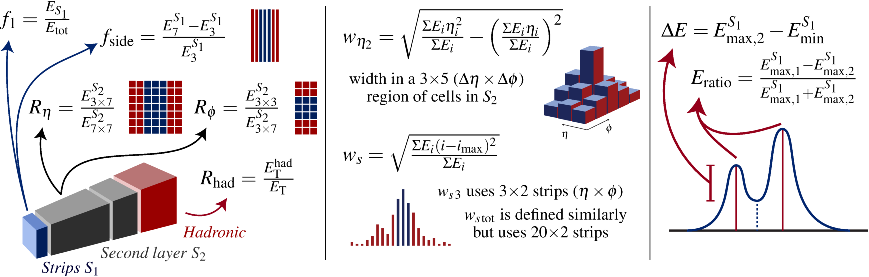
\includegraphics[width=\linewidth]{4_photonid/introduction/diagrams/shower-shapes}
    \caption{Representación esquemática de las \ac{SS} de fotones.}
    \label{fig:pid_ss:ss:ss_variables}
\end{figure}

A continuación se detallan las \acp{SS} utilizadas para la identificación de fotones que se muestran resumidas en \Tab{\ref{tab:pid_ss:ss:ss_variables}} y un esquema de cómo son calculadas se encuentra en la \Fig{\ref{fig:pid_ss:ss:ss_variables}}.
Las primeras variables hacen uso de la energía medida en el \ac{HCAL}:
\begin{itemize}
    \item Filtración hadrónica: es la energía transversal depositada en el \ac{HCAL}, normalizada respecto a la energía depositada en el \ac{ECAL}:
        \begin{equation}
            {\rhad}_{(1)} = \frac{\et^{\text{HCAL}}}{\et^{\text{ECAL}}}
        \end{equation}
        Para minimizar los efectos de la degradación de la resolución, en la región de transición barrel-endcap del \ac{HCAL} (\(0.8\leq \abseta\leq 1.37\)) se utiliza la energía depositada en todo el \ac{HCAL} (\rhad). En el resto del detector, sólo se utiliza la energía depositada en la primera capa del \ac{HCAL} (\rhado).
\end{itemize}
Las siguientes variables utilizan la información de la segunda capa del \ac{ECAL}:
\begin{itemize}
    \item Perfil de energía lateral en \(\eta\):
        \begin{equation}
            \reta = \frac{E_{3\times7}^{s2}}{E_{7\times7}^{s2}}
        \end{equation}
        donde \(E_{i\times j}^{s2}\) es la suma de energía en la segunda capa del calorímetro contenida en una ventana de \(i \times j \) celdas (unidades de \(\eta \times \phi\)) centrada en la celda más energética. Esta variable da una medida del ancho de las lluvias en la dirección \(\eta\).
    \item Perfil de energía lateral en \(\phi\):
        \begin{equation}
            \rphi = \frac{E_{3\times3}^{s2}}{E_{3\times7}^{s2}}
        \end{equation}
        definida de forma similar a \reta. Sin embargo, esta variable se comporta de forma muy diferente para fotones convertidos y no convertidos. Debido a la acción del campo magnético, los electrones y positrones se curvan en direcciones opuestas en \(\phi\), por lo que se producen lluvias \ac{EM} más anchas para los fotones convertidos que para los no convertidos.
    \item Ancho de la lluvia lateral en \(\eta\):
        \begin{equation}
            \weta = \sqrt{
                \frac{\sum E_i \eta_i^2}{\sum E_i}
                -
                \left(\frac{\sum E_i \eta_i}{\sum E_i}\right)^2
            }
        \end{equation}
        mide el ancho propio de la lluvia \ac{EM}, donde \(E_i\) es la energía en la \(i\)-ésima celda del \ac{ECAL}, medida en una ventana de \(3\times 5 \) celdas en \(\eta \times \phi\).
\end{itemize}
Las siguientes variables utilizan la información de la primera capa del \ac{ECAL}, compuesta por las celdas \textit{strips} que permiten una alta resolución en \(\eta\) y permite una buena separación entre fotones aislados de fotones producto del decaimiento de \(\pizero\). La \Fig{\ref{fig:pid_ss:ss:pizero}} muestra la diferencia en la energía depositada en el \ac{ECAL} entre los dos casos mencionados anteriormente.
\begin{itemize}
    \item Perfil de energía lateral en \(\eta\):
        \begin{equation}
            \fside = \frac{E_7^{s1} - E_3^{s1}}{E_3^{s1}}
        \end{equation}
        mide la energía fuera del núcleo de las tres strips centrales dentro de una ventana de 7 celdas, dividida por la energía en las tres celdas centrales.
    \item Ancho de la lluvia lateral en \(\eta\) (3 strips)
        \begin{equation}
            \wone = \sqrt{
                \frac{\sum E_i (i - i_{max})^2}{\sum E_i}
            }
        \end{equation}
        donde \(i\) corre sobre todas las celdas en una ventana de 3 celdas alrededor de la de mayor energía. Esta variable mide el ancho de la lluvia \ac{EM} en la primera capa del calorímetro.
    \item Ancho de la lluvia lateral en \(\eta\) (total).
        Se define de forma similar a \wone pero utilizando todas las celdas en una ventana de \(\Delta\eta\times\Delta\phi=0.0625\times 0.2\), que corresponde aproximadamente a \(20\times 2\) strips en \(\eta\times\phi\).
    \item Diferencia energética
        \begin{equation}
            \deltae = E_{\text{max}, 2}^{s1} - E_{\text{min}}^{s1}
        \end{equation}
        representa la diferencia de energía entre el segundo máximo y la energía mínima reconstruida entre los dos máximos de la primera capa del \ac{ECAL}.
    \item Asimetría de energía
        \begin{equation}
            \eratio = \frac{
                E_{\text{max}, 1}^{s1} - E_{\text{max}, 2}^{s1}
            }{
                E_{\text{max}, 1}^{s1} + E_{\text{max}, 2}^{s1}
            }
        \end{equation}
        es la relación de la diferencia de energía entre los dos máximos, normalizada con respecto a la suma de esas energías, en la primera capa del \ac{ECAL}.
\end{itemize}

\begin{figure}[ht!]
    \centering
    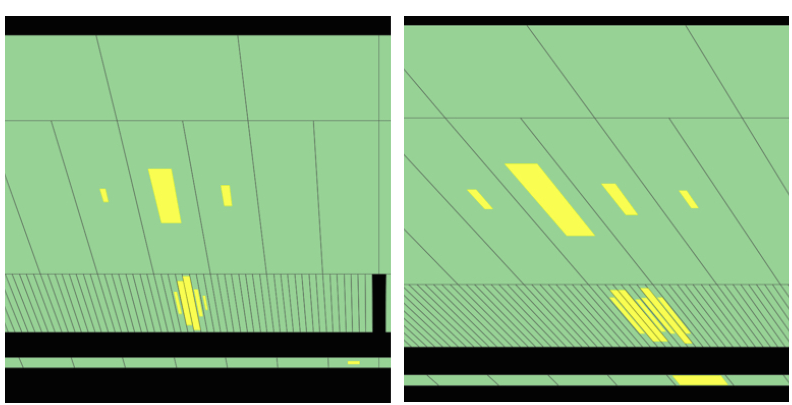
\includegraphics[width=0.7\linewidth]{4_photonid/introduction/diagrams/PhotonPizero}
    \caption{Depósitos de energía característicos para un fotón aislado (izquierda), y un evento \(\pizero\to\gamma\gamma\) (derecha), que es posible distinguir gracias a la fina granularidad de la primera capa del \ac{ECAL}~\cite{ATLAS-ECAL-Pizero}.}
    \label{fig:pid_ss:ss:pizero}
\end{figure}






\section{Identificación de fotones}
\label{sec:pid_ss:pid}

La identificación de fotones prompt frente a fotones falsos en colisiones hadrónicas es un gran desafío. Los fotones falsos están ampliamente dominados por candidatos a fotones que surgen del decaimiento de hadrones (mayormente piones neutros) en fotones, mientras que una fracción más pequeña de candidatos falsos está asociada con otras partículas que depositan una energía significativa en el \ac{ECAL}, imitando la de los fotones reales.
Tanto para las búsquedas como para las medidas de precisión es importante contar con algoritmos y técnicas para identificar los fotones reales frente a los falsos. Estas búsquedas o medidas de precisión se llevan a cabo en un rango muy amplio de energía del fotón empezando por resonancias de baja masa, por ejemplo, con un Higgs decayendo a un par de partículas tipo axión que decaen en 4 fotones (\(\PH\to aa \to 4\gamma\))~\cite{ATLAS-HiggsTo4Gamma} donde el momento transverso del fotón es de \(\sim 25~\gev\), hasta fotones de muy alto \pt en búsquedas de resonancias \gammajet como los que se realizan para esta tesis, donde los fotones tienen un momento transverso mayor a \(1~\tev\) (\Part{\ref{part:search}}).

La identificación de fotones en \ac{ATLAS} está basada en cortes en las \acp{SS} y que permite definir diferentes \acfp{WP} con diferentes características: ya sea lograr un gran rechazo de fondo o alta eficiencia de señal, o simplemente bajos tiempos de cómputo para la identificación \textit{online}. En esta sección se describe el procedimiento utilizado para la optimización de estos \acp{WP} y luego se describen los métodos para medir las eficiencias correspondientes.



\subsection{Procesos de interés y selección de eventos}
\label{subsec:pid_ss:pid:event_selection}

Dado el amplio rango de energías en el que se utilizan los fotones en \ac{ATLAS}, para la optimización de los \acp{WP} se utilizan dos procesos diferentes que permiten obtener muestras limpias de fotones en los regímenes de bajo y alto \pt. En el caso de bajo \pt, se utiliza una fuente muy limpia de fotones procedentes de decaimientos radiativos del bosón \Zboson. Por otro lado, aunque con mayor contaminación de fondo, se emplean eventos de fotones prompt (ver la \Sect{\ref{subsec:theory:sm:prompt_photon}}) para fotones de alto \pt. En los siguientes párrafos se ofrece una descripción de cada de las muestras de fotones utilizadas.


\paragraph{Decaimientos radiativos del bosón \Zboson}

Hay dos modos de producción posibles para los procesos del \ac{SM} de \(\pp\to \Zboson(\ellell)\gamma\), donde \(\ell\) es un electrón o un muón. Estos son: \acf{ISR} donde el fotón es radiado por los quarks y \acf{FSR}, donde el fotón es radiado por uno de los leptones del estado final a través de bremsstrahlung. Ambos modos de producción se muestran en la \Fig{\ref{fig:pid_ss:event_selection:fsr_isr}}.


\begin{figure}[ht!]
    \centering
    \begin{subfigure}[h]{0.49\linewidth}
        \centering
        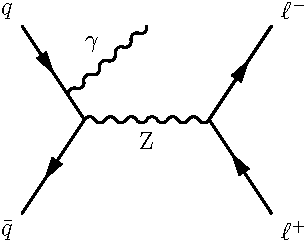
\includegraphics[width=0.6\linewidth]{4_photonid/introduction/diagrams/isr}
        \caption{\Acf{ISR}}
    \end{subfigure}
    \hfill
    \begin{subfigure}[h]{0.49\linewidth}
        \centering
        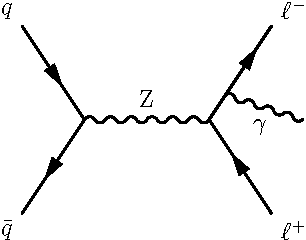
\includegraphics[width=0.6\linewidth]{4_photonid/introduction/diagrams/fsr}
        \caption{\Acf{FSR}}
    \end{subfigure}
    \caption{Diagrams de Feynman del proceso de radiación de un fotón en decaimientos \(\Zboson\to\ell\ell\gamma\) para los casos de \ac{ISR} (izquierda) y \ac{FSR} (derecha).}
    \label{fig:pid_ss:event_selection:fsr_isr}
\end{figure}


Ambos procesos \ac{FSR} y \ac{ISR} pueden identificarse fácilmente comparando la distribución de la masa invariante de los dos leptones (\mll) con la distribución de la masa invariante de los dos leptones junto con el fotón (\mlly).
Para los eventos \ac{ISR}, \mll tiene su máximo en el valor de la masa del \Zboson y el fotón simplemente suma a la masa invariante de tres cuerpos (\mlly) haciéndola mayor que \(\sim 91~\gev\). En el caso \ac{FSR}, en cambio, la masa invariante de tres cuerpos \mlly presenta su máximo en el valor de la masa del \Zboson.
% , observado en la \Fig{\ref{fig:pid_ss:event_selection:mll_mlly_distribution:data}}.
Para los estudios de identificación de fotones sólo se consideran los fotones de los eventos \ac{FSR} (de ahora en más también referido como decaimiento \acf{RZ}). Los eventos \ac{ISR} también sufren la contaminación de fondos provenientes de eventos \Zjets, en los que el jet se identifica erróneamente como un fotón y además la sección eficaz \Zjets es de varios órdenes de magnitud mayor a la del proceso \(\Zboson+\gamma\). A partir de las \Figs{\ref{fig:pid_ss:event_selection:mll_mlly_distribution:bkg}}{\ref{fig:pid_ss:event_selection:mll_mlly_distribution:signal}} donde se muestran las distribuciones de \mll en función de \mlly para los procesos simulados de \(\Zboson\to\ell\ell\) y \(\Zboson\to\ell\ell\gamma\), respectivamente, se puede apreciar la separación entre estos dos procesos cuando se seleccionan fotones \ac{FSR}.

\begin{figure}[ht!]
    \centering
    \begin{subfigure}[h]{0.32\linewidth}
        \centering
        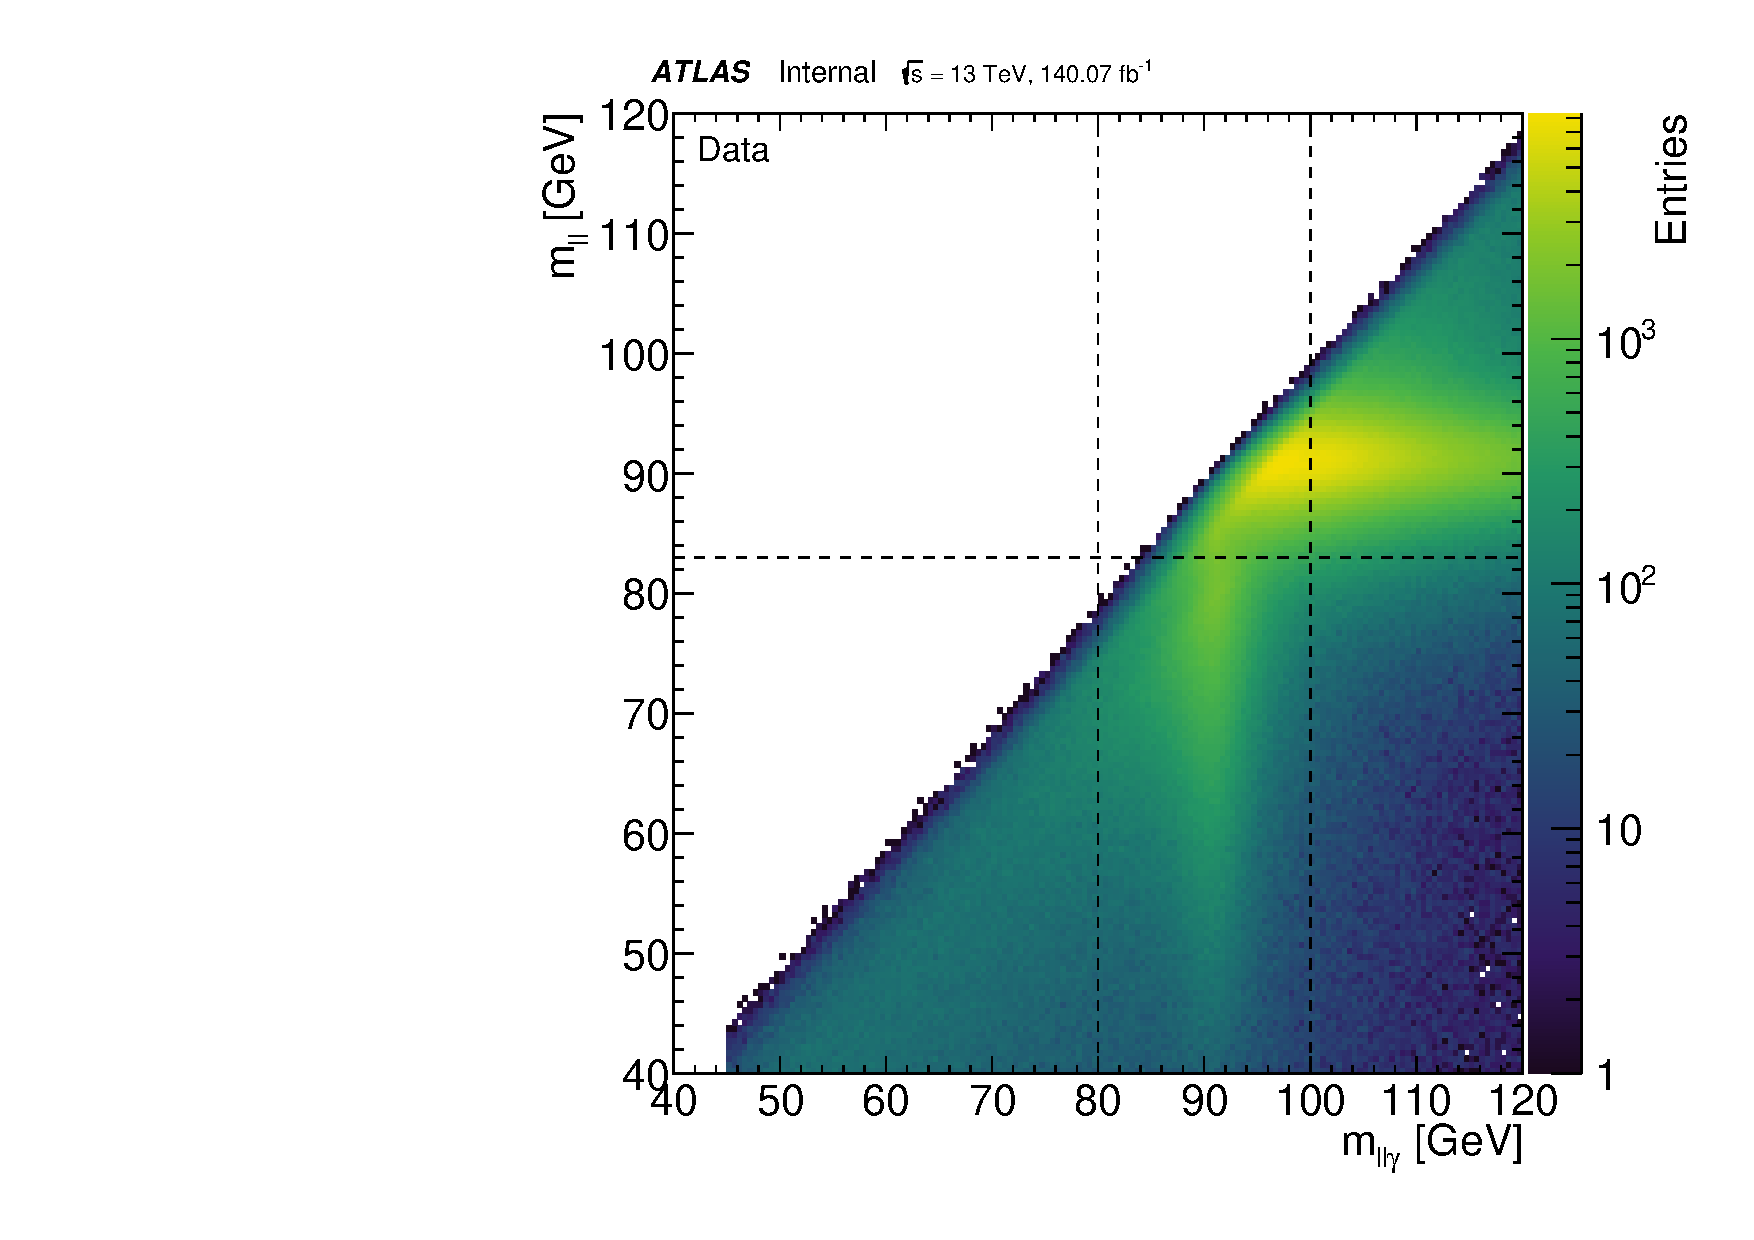
\includegraphics[width=\linewidth]{4_photonid/introduction/can2d__data__nosel__llg_m_ll_m__RZ__rel22_run2_Run2}
        \caption{Data}
        \label{fig:pid_ss:event_selection:mll_mlly_distribution:data}
    \end{subfigure}
    \hfill
    \begin{subfigure}[h]{0.32\linewidth}
        \centering
        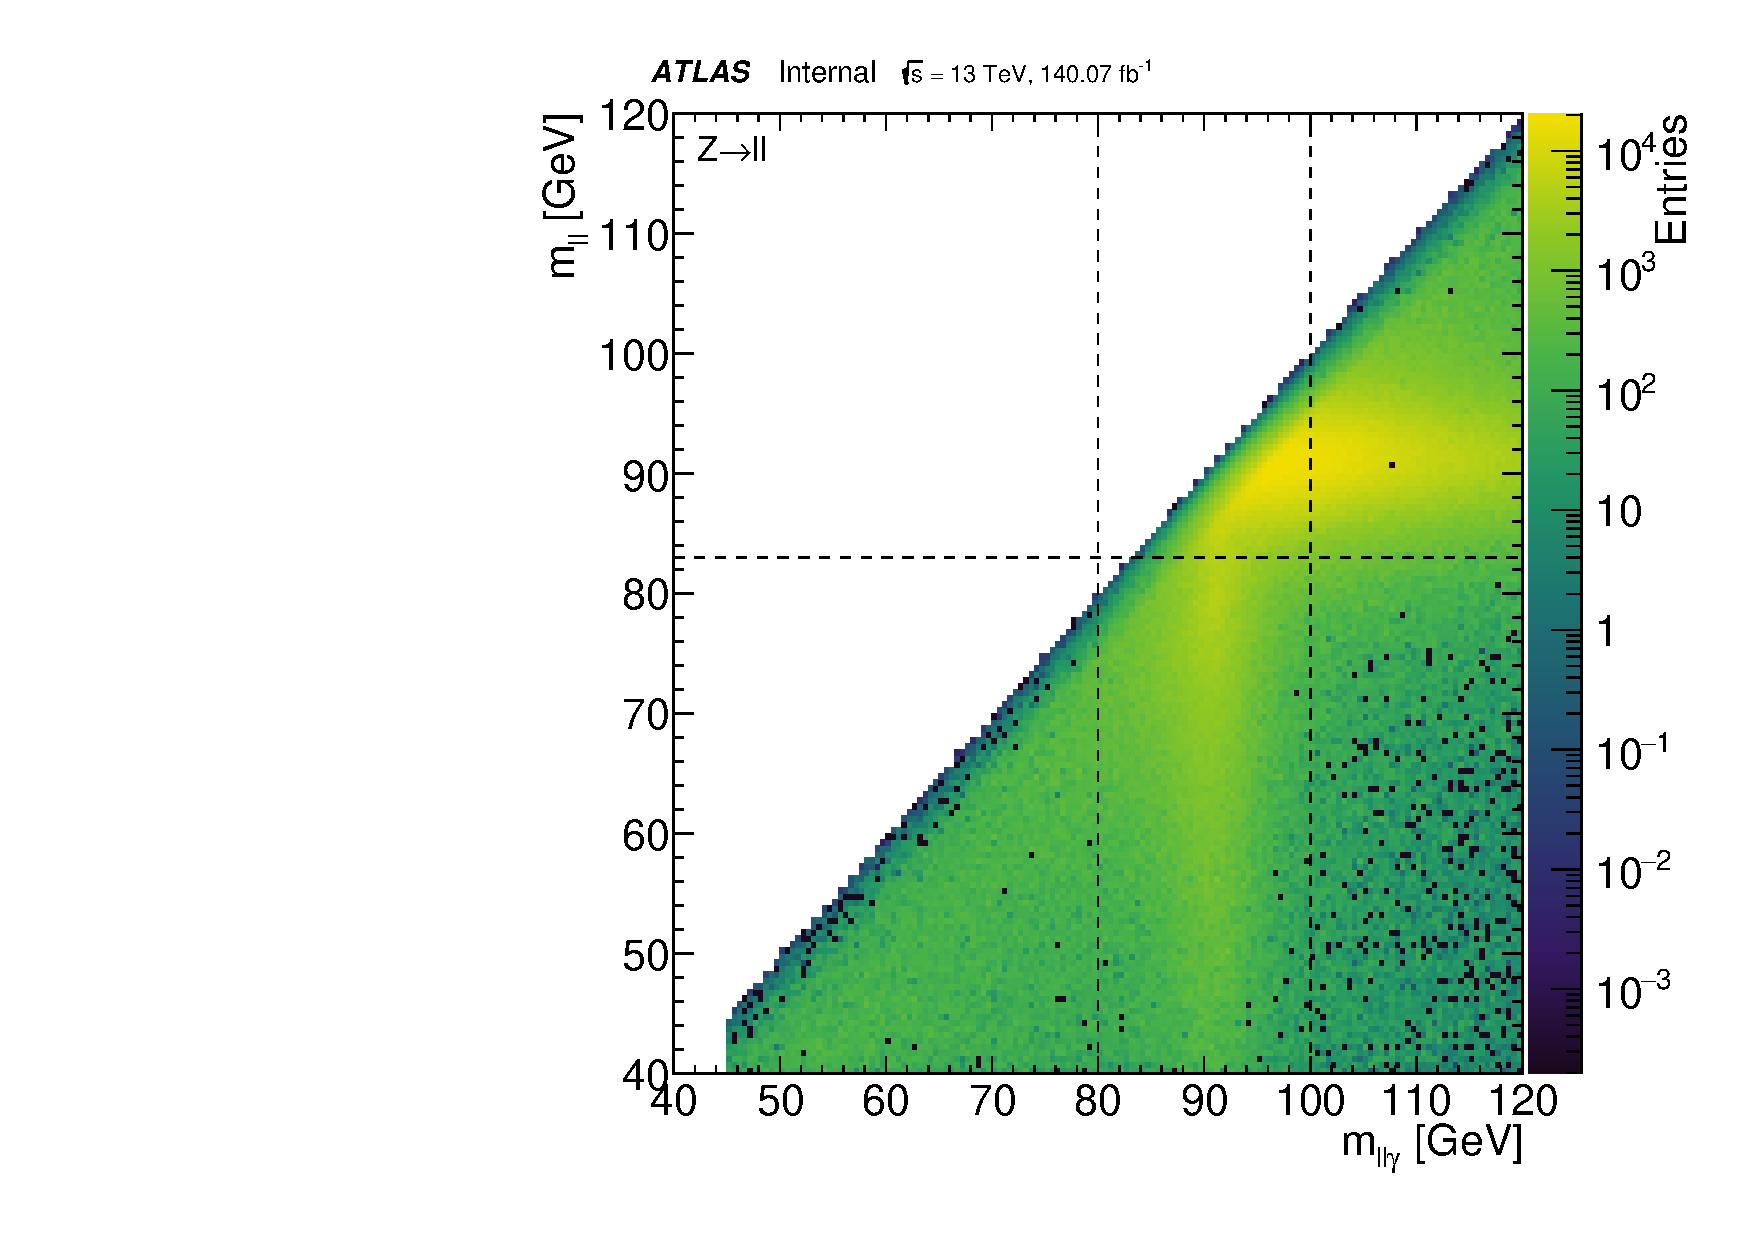
\includegraphics[width=\linewidth]{4_photonid/introduction/can2d__bkg__nosel__llg_m_ll_m__RZ__rel22_run2_Run2}
        \caption{\(\Zboson\to \ell\ell\)}
        \label{fig:pid_ss:event_selection:mll_mlly_distribution:bkg}
    \end{subfigure}
    \hfill
    \begin{subfigure}[h]{0.32\linewidth}
        \centering
        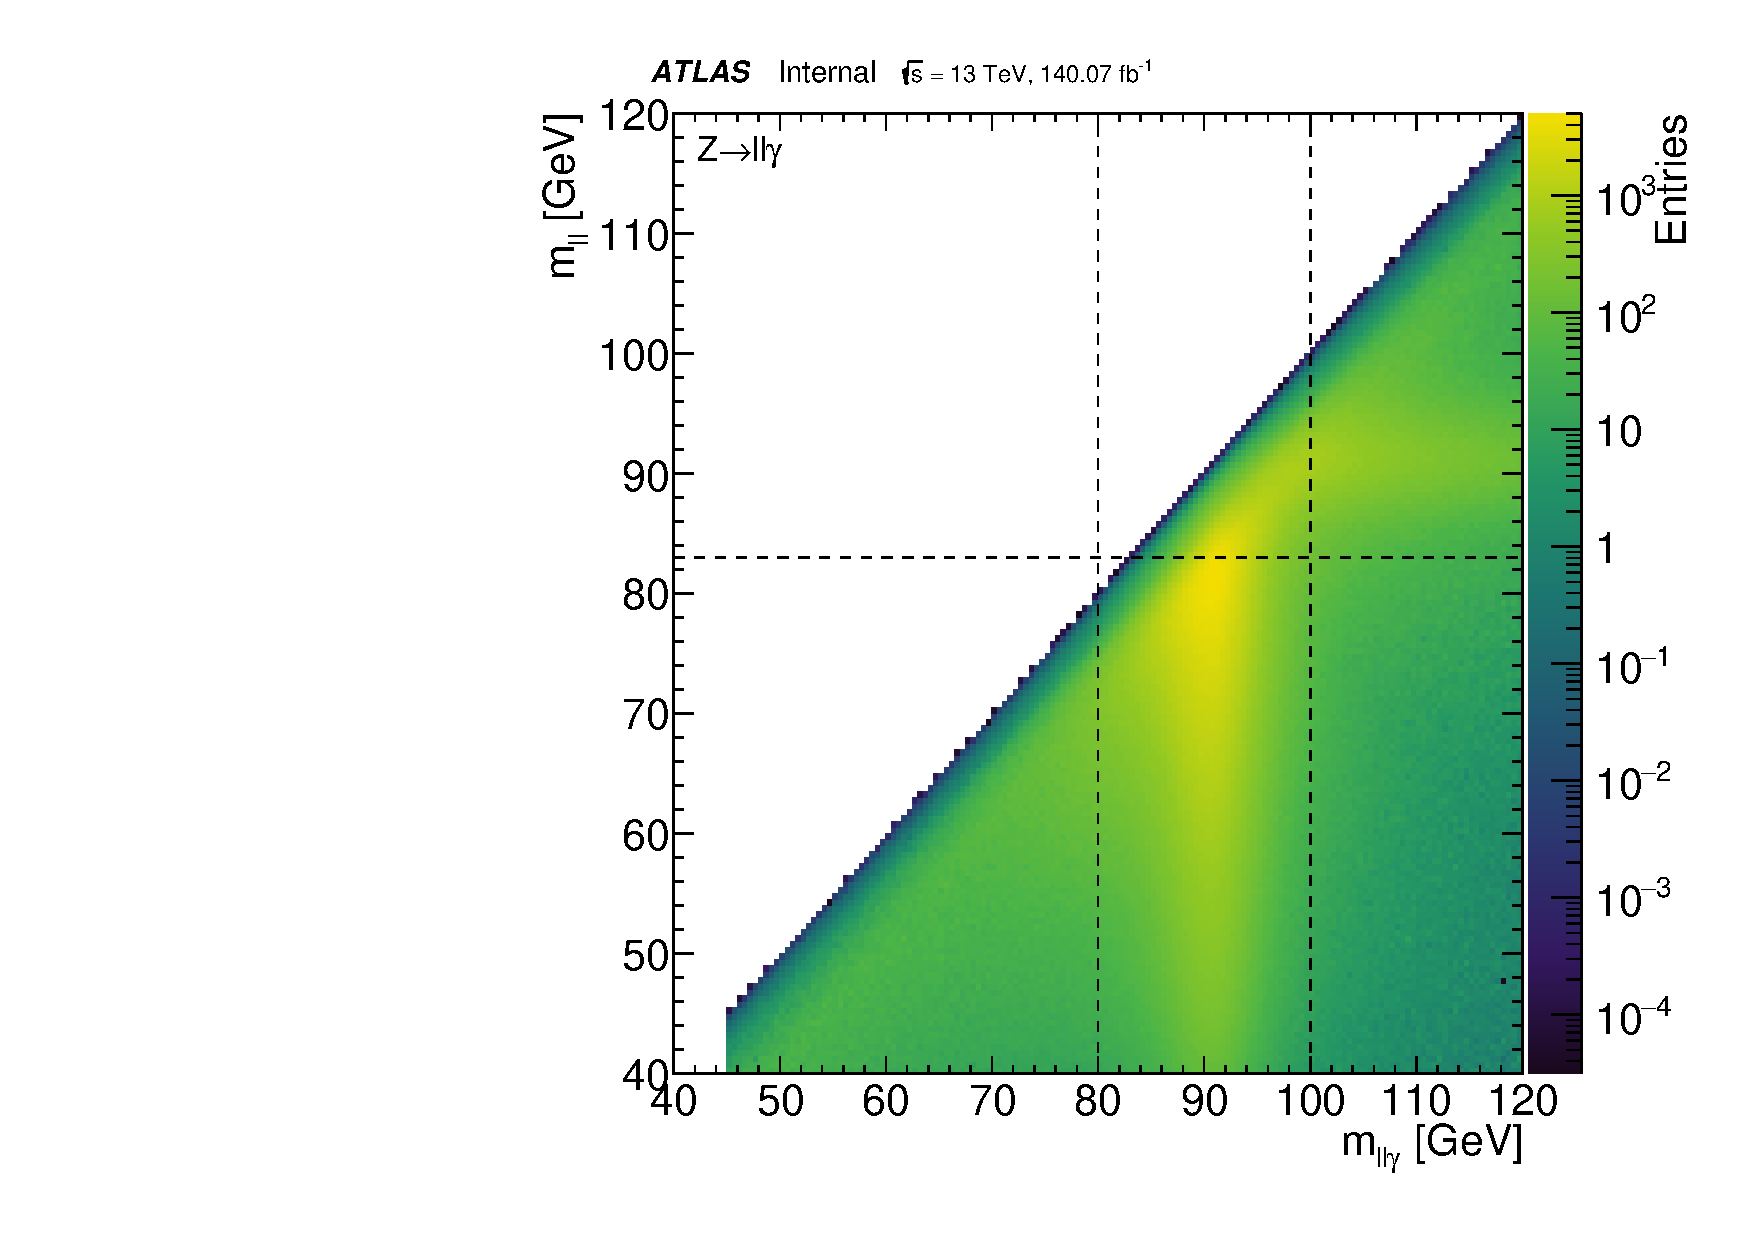
\includegraphics[width=\linewidth]{4_photonid/introduction/can2d__signal__nosel__llg_m_ll_m__RZ__rel22_run2_Run2}
        \caption{\(\Zboson\to \ell\ell\gamma\)}
        \label{fig:pid_ss:event_selection:mll_mlly_distribution:signal}
    \end{subfigure}
    \caption{Masa invariante de los dos leptones en función de la masa invariante de ambos leptones junto con un fotón en (\subref{fig:pid_ss:event_selection:mll_mlly_distribution:data}) datos, (\subref{fig:pid_ss:event_selection:mll_mlly_distribution:bkg}) fondos y (\subref{fig:pid_ss:event_selection:mll_mlly_distribution:signal}) señal. La región en la cual se encuentra una gran concentración de eventos con \(m_{\ell\ell} \sim m_{\Zboson}\) corresponde a eventos de \ac{ISR}, mientras que eventos de \ac{FSR} events están caracterizados por \(m_{\ell\ell\gamma} \sim m_{\Zboson}\).}
    \label{fig:pid_ss:event_selection:mll_mlly_distribution}
\end{figure}

Se requiere que los fotones tengan un momento transverso \(\pt>7~\gev\) y una pseudorapidez en el rango de \(\abseta<1.37\) o \(1.52<\abseta<2.37\), evitando así la región del crack.
Para los estudios de optimización no se aplica ningún requisito de aislamiento sobre los fotones, pero para las medidas de eficiencia se utiliza el \ac{WP} de aislamiento \texttt{Loose}, descripto en la \Sect{\ref{subsec:objects:egamma:iso}}. Se requiere que los leptones tengan \(\et>10~\gev\), los muones una pseudorapidez \(\abseta<2.5\) y para los electrones \(\abseta<2.47\), excluyendo el crack. Tanto a los electrones como a los muones se les exige que pasen los requisitos de aislamiento \texttt{Loose} y que pasen el criterio de identificación \texttt{Medium}.

El fotón \ac{FSR} se selecciona entonces requiriendo \(80<\mlly<100~\gev\) y \(40<\mll<83~\gev\). Finalmente, para evitar cualquier sesgo en las \ac{SS} del fotón y en sus variables de aislamiento, se requiere una distancia mínima de \(\DeltaR>0.4\) entre dicho fotón y el leptón más cercano.


\paragraph{\acf{SP}}

La muestra de fotones inclusivos, o \acf{SP}, se recoge mediante triggers que requieren un sólo fotón con umbrales que varían entre \(10~\gev\) y \(140~\gev\) e identificación \texttt{Loose}. Aunque los triggers utilizados para obtener esta muestra están preescalados (con la excepción del de \(140~\gev\)), proporcionan un gran conjuntos de datos de fotones de alto \pt.
Estos procesos incluyen eventos a \ac{LO} de \gammajet procedentes de la dispersión dura \(qg\to q\gamma\) y \(\qqbar \to g\gamma\), así como fotones prompt procedentes de la fragmentación de quarks en eventos de dijet de \acs{QCD}.
Se requiere que estos fotones presenten una pseudorapidez de \(\abseta<2.37\) excluyendo el crack, y pasar el requisito de aislamiento \texttt{Loose}. Las muestras de \ac{SP} se utilizan tanto para los estudios de optimización como para la estimación de las eficiencias.


\subsection{Optimización}
\label{subsec:pid_ss:pid:optimisation}

A partir de las \acp{SS} anteriormente descriptas se definen tres \acp{WP} para los fotones: \texttt{Loose}, \texttt{Medium} y \texttt{Tight}~\cite{ATLAS-EGamma-Performance-2024}. El \ac{WP} loose emplea cortes a las variables definidas en la segunda capa y a la variable de filtración hadrónica y es utilizado principalmente por el trigger.
Los \acp{WP} medium y tight utilizan todas las variables definidas previamente. El \ac{WP} medium está optimizado para tener una eficiencia fija de \(95\%\), mientras que el \ac{WP} tight proporciona un excelente rechazo de fondo. La \Tab{\ref{tab:pid_ss:ss:ss_variables}} muestra qué variables se utilizan para cada \ac{WP}.

Para la optimización de los \acp{WP} se utilizan las dos muestras definidas previamente: los eventos \ac{RZ} para fotones con \(10<\pt<25~\gev\) como señales y eventos de \(\Zboson\to \ell\ell\) como fondos; y para el régimen de alto \pt (\(\pt>25~\gev\)) los eventos de \ac{SP} se consideran como señal mientras que los eventos dijet son los fondos.

En la \Fig{\ref{fig:pid_ss:optimisation:shower_shapes}} se muestran ejemplos de tres de estas \ac{SS} (\reta, \eratio y \weta) comparando eventos de señal y de fondo utilizando las muestras de \ac{RZ}, donde se observa un excelente poder discriminatorio.
Los cortes en todas las \acp{SS} para cada \ac{WP} de identificación se obtienen en función de la energía transversal y la pseudo-rapidez del candidato a fotón, para tener en cuenta la forma de las variables para diferentes \(\eta\) y para variaciones en la cantidad de material y la geometría del calorímetro. Los \acp{WP} medium y tight también se calculan por separado para fotones convertidos y no convertidos.
Los cortes se optimizan utilizando un enfoque multivariable en el que las eficiencias de señal se escanean entre \(0\%\) y \(100\%\) mientras se intenta maximizar el rechazo de fondo.

\begin{figure}[ht!]
    \centering
    \begin{subfigure}[h]{0.32\linewidth}
        \centering
        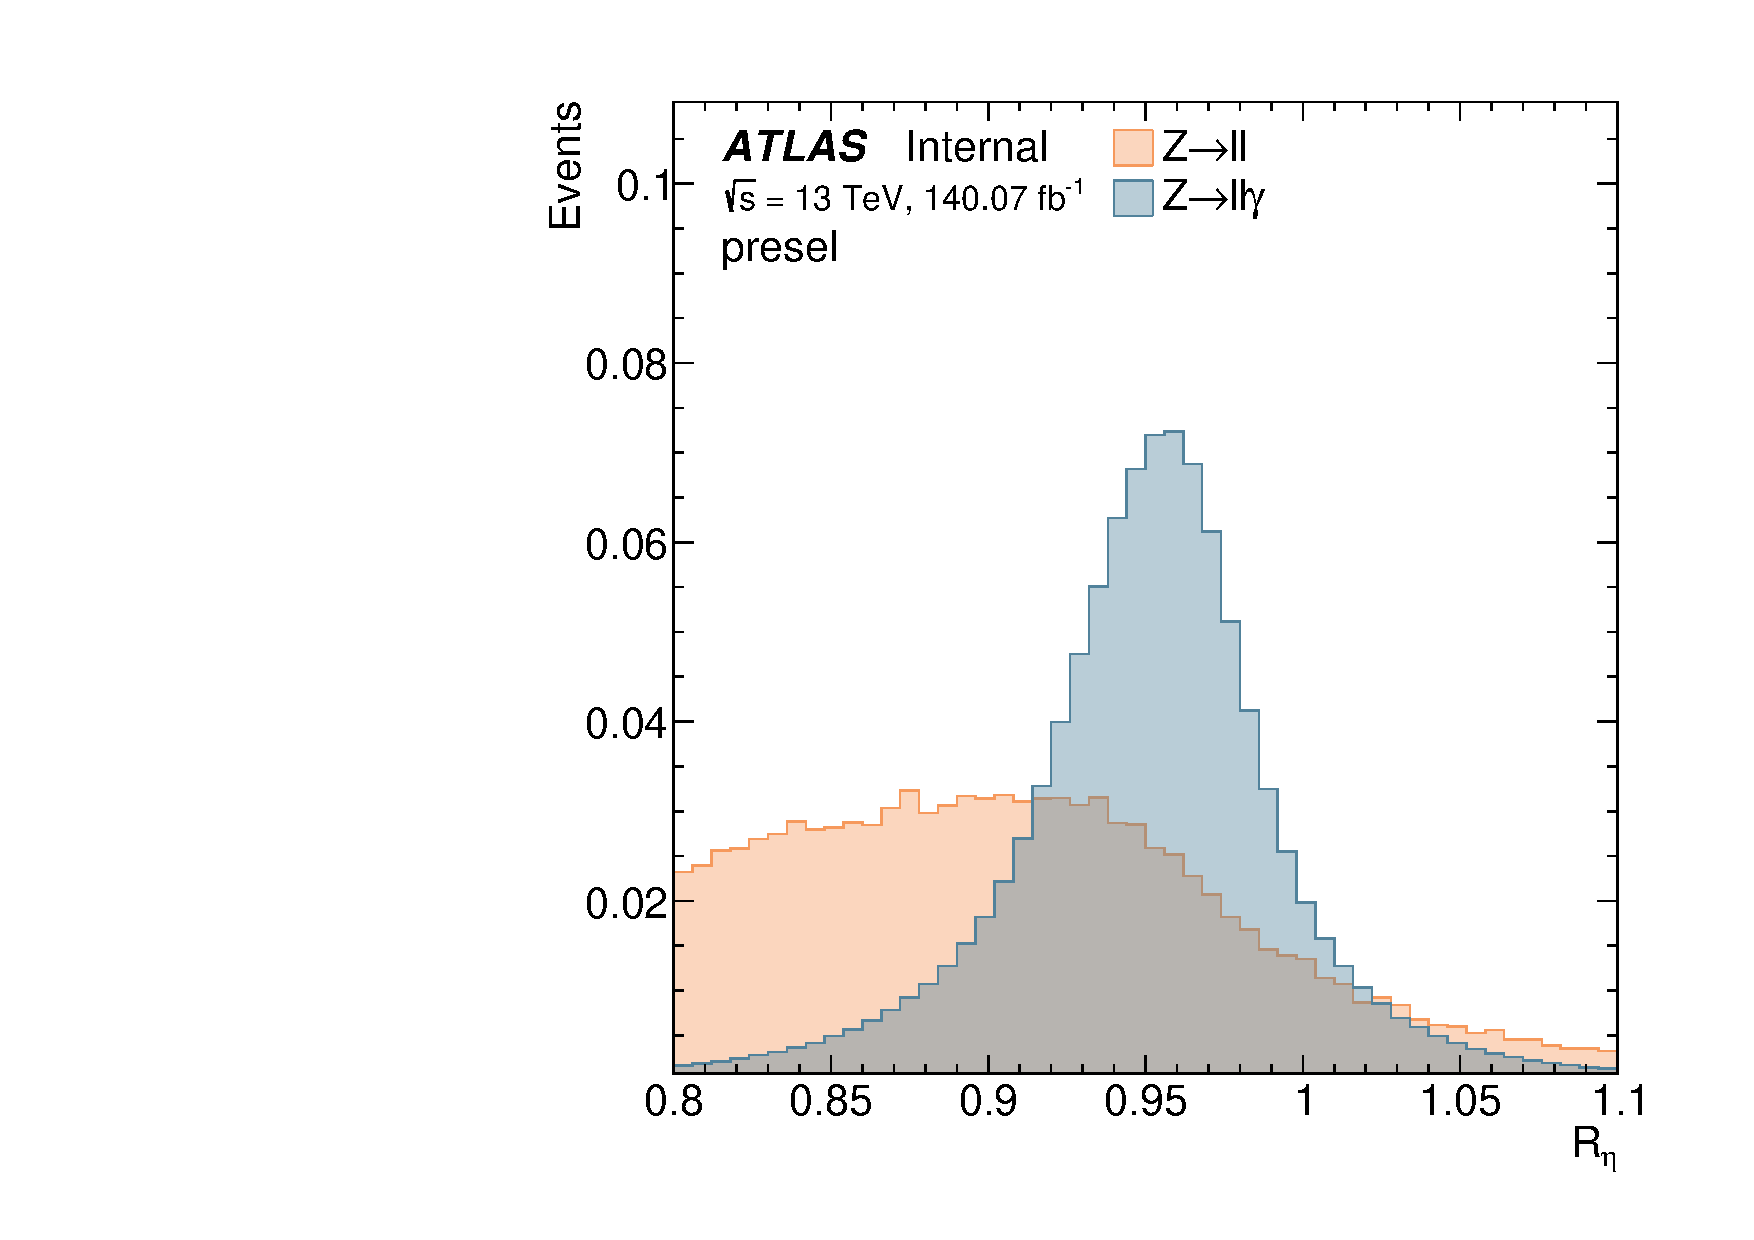
\includegraphics[width=\linewidth]{4_photonid/introduction/shower_shapes/can__sigbkg__presel__ph_reta__RZ__rel22_run2_Run2}
        \caption{\reta}
        \label{fig:pid_ss:optimisation:shower_shapes:reta}
    \end{subfigure}
    \hfill
    \begin{subfigure}[h]{0.32\linewidth}
        \centering
        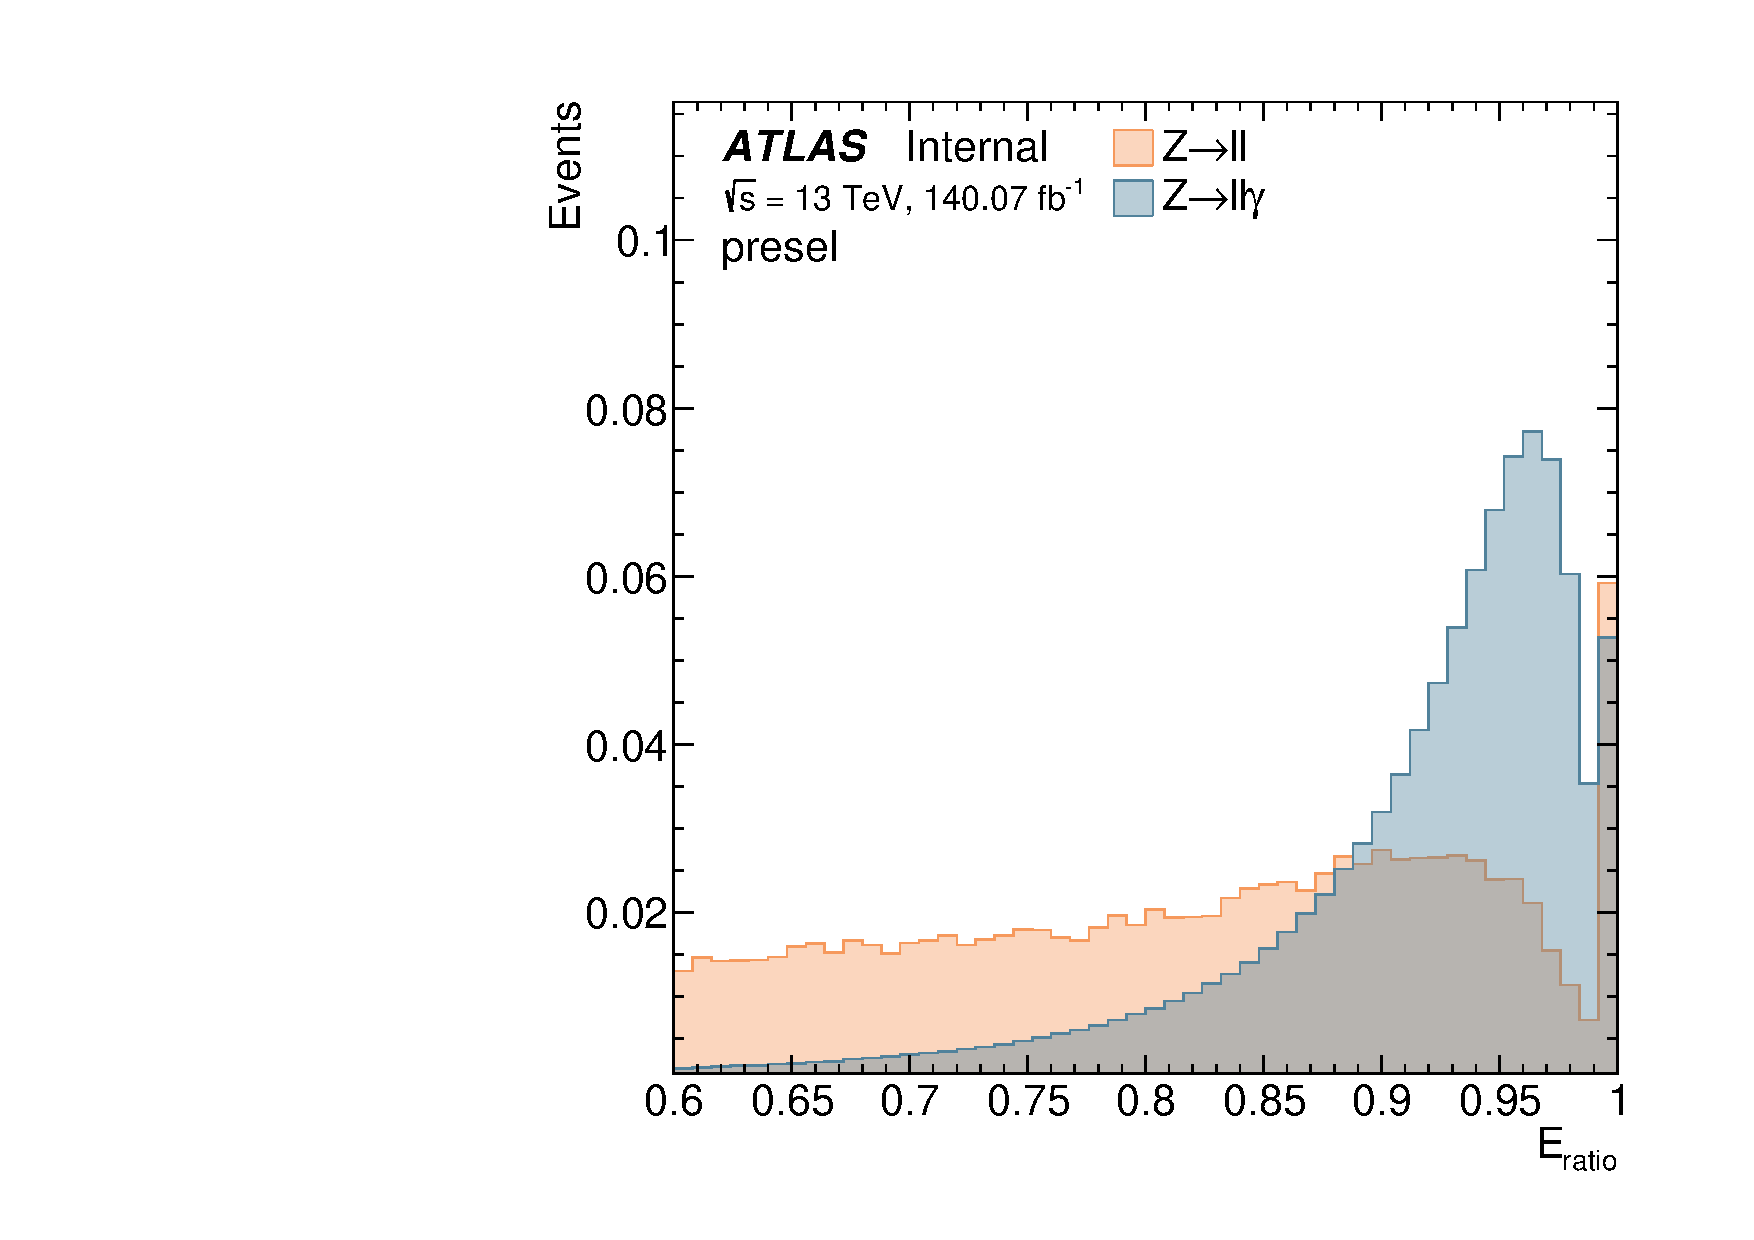
\includegraphics[width=\linewidth]{4_photonid/introduction/shower_shapes/can__sigbkg__presel__ph_eratio__RZ__rel22_run2_Run2}
        \caption{\eratio}
        \label{fig:pid_ss:optimisation:shower_shapes:eratio}
    \end{subfigure}
    \hfill
    \begin{subfigure}[h]{0.32\linewidth}
        \centering
        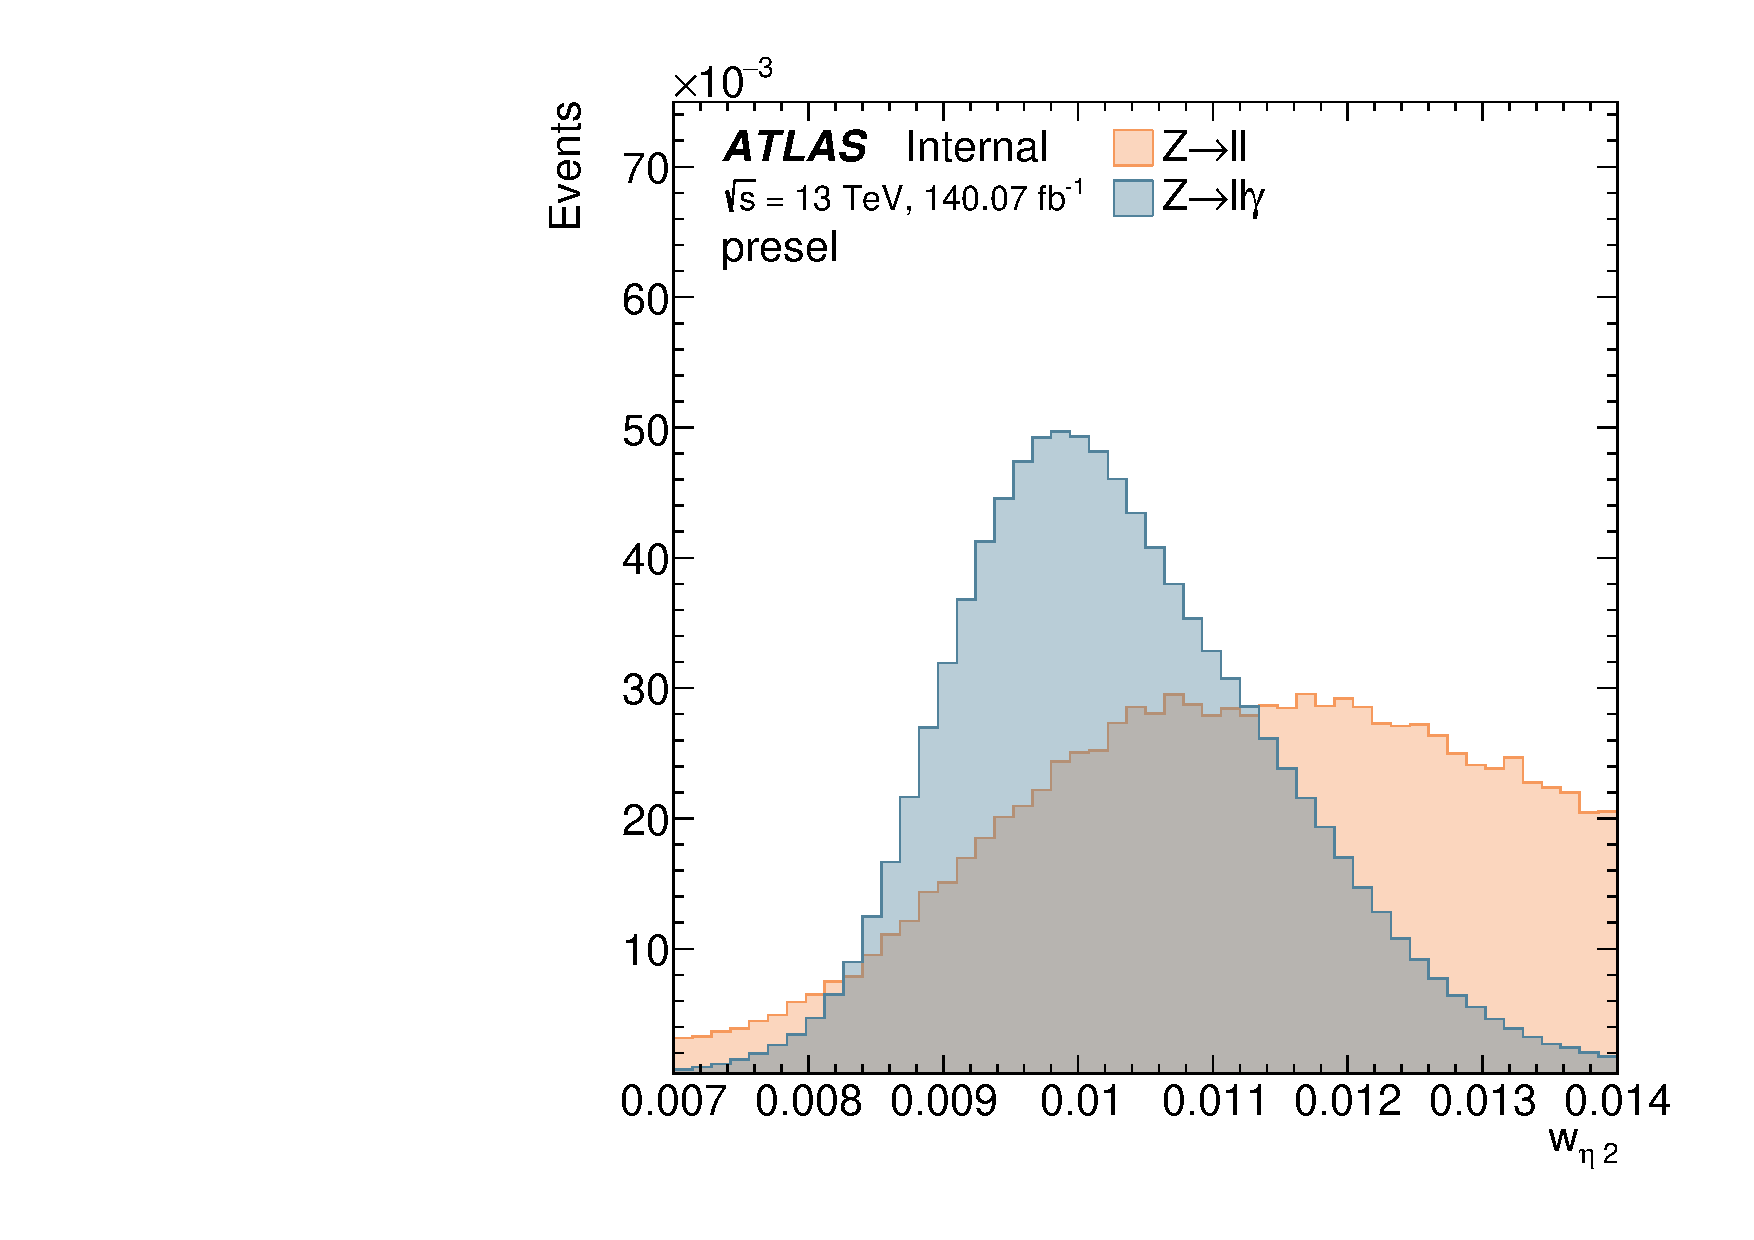
\includegraphics[width=\linewidth]{4_photonid/introduction/shower_shapes/can__sigbkg__presel__ph_weta2__RZ__rel22_run2_Run2}
        \caption{\weta}
        \label{fig:pid_ss:optimisation:shower_shapes:weta2}
    \end{subfigure}
    \caption{Distribuciones normalizadas de señal (azul) y fondo (naranja) de diferentes \acp{SS} utilizando las muestras de \ac{RZ} y pasando la selección de eventos detallada en la \Sect{\ref{subsec:pid_ss:pid:event_selection}}.}
    \label{fig:pid_ss:optimisation:shower_shapes}
\end{figure}



\subsection{Estimación de las eficiencias}

Una vez optimizados los diversos \acp{WP} de identificación es fundamental estimar las eficiencias de los datos y las simulaciones \ac{MC}. Las estimaciones de eficiencias de fotones se realizan utilizando tres métodos diferentes en diferentes rangos de \pt, que son detallados en la \Refn{\cite{ATLAS-EGamma-Performance-2015-2016}} y son brevemente descriptos en los próximos párrafos.
Para los tres métodos se requiere que los fotones satisfagan el criterio de aislamiento loose definido en la \Sect{\ref{subsec:objects:egamma:iso}} y, por tanto, las eficiencias de identificación de los fotones se miden con respecto a este criterio de aislamiento. 

Para el rango de bajo \pt (\(7<\pt<100~\gev\)), los fotones procedentes del proceso \ac{RZ} se utilizan como fotones de señal. El método para estimar las eficiencias consiste en ajustar la distribución observada de la masa invariante de tres cuerpos (\mlly) antes y después de aplicar el criterio de identificación tight. El número de eventos de señal y de fondo puede estimarse a partir de los ajustes y las purezas de señal se calculan antes (\(P^{\text{total}}\)) y después (\(P^{\text{pass}}\)) de la aplicación de la identificación tight.
La eficiencia final en los datos viene dada por:
\begin{equation*}
    \varepsilon_{ID} = \frac{ P^{\text{pass}} N_{\text{data}}^{\text{pass}} }{ P^{\text{total}} N_{\text{data}}^{\text{total}} }.
\end{equation*}

El segundo método para calcular eficiencias consiste en aplicar transformaciones de Smirnov~\cite{SmirnovTransform} para que las distribuciones de las \acp{SS} de los electrones se parezcan a las de los fotones. Las muestras usadas en este método son simulaciones de decaimientos \(\Zboson\to ee\), en los que se requiere que los electrones pasen el criterio de aislamiento de fotones loose. También es necesario tener en cuenta la contribución de una pequeña fracción de fondo de procesos \Wjets y producción multijet. Estos fondos son tratados mediante ajustes a la distribución de \(m_{ee}\) de datos, utilizando señales simuladas y formas funcionales que describen el restos de los fondos, obtenidas en regiones de control (regiones en donde las contribuciones de estos fondos son dominantes y separables). Luego, los candidatos a electrones se cuentan a partir de eventos en el rango \(70 < m_{ee} < 110~\gev\) y las eficiencias se miden utilizando el método tag-and-probe descripto en la \Refn{\cite{ATLAS-EGamma-Performance-2015-2017}}. El rango \pt en el que se aplica este método es \(25<\pt<250~\gev\).

El último y tercer método utiliza muestras de \ac{SP} con fotones en el rango \(50<\pt<1500~\gev\). En este caso se utiliza el \textit{Matrix Method}~\cite{ATLAS-EGamma-Performance-2015-2016} que construye cuatro regiones ortogonales que pasan o no el \ac{WP} de identificación tight y pasan o no el aislamiento de trazas (descripto en la \Sect{\ref{subsec:objects:egamma:iso}}). Para cada región surgen dos incógnitas: el número de eventos de señal y de fondo.
Si se conocen las eficiencias de aislamiento de trazas para los componentes de señal y de fondo, entonces es posible estimar la eficiencia de los fotones loose que pasan los criterios de identificación tight. Las eficiencias de aislamiento para los fotones de señal se estiman utilizando muestras de \ac{MC} y las de fondo se obtienen en una región de control enriquecida con jets construida a partir de la inversión de los criterios de identificación.
Las eficiencias en datos para el \ac{WP} de identificación tight son entonces:
\begin{equation*}
    \varepsilon^{\text{tight-ID}} = \frac{
        \frac{
            \hat{\varepsilon}_{\text{ID}} - \hat{\varepsilon}_{\text{ID}}^b
        }{
            \hat{\varepsilon}_{\text{ID}}^s - \hat{\varepsilon}_{\text{ID}}^b
        }
        \cdot
        N_{\text{ID}}^T
    }{
        \frac{
            \hat{\varepsilon} - \hat{\varepsilon}^b
        }{
            \hat{\varepsilon}^s - \hat{\varepsilon}^b
        }
        \cdot
        N^T
    },
\end{equation*}
donde \(N^T\) representa la totalidad de fotones en la muestra inclusiva que consiste en \(N^s\) fotones de señal (o fotones prompt) y \(N^b\) fotones falsos (fotones de fondo). El número \(N^T_{\text{ID}}\) es el subconjunto de \(N^T\) que pasa el requisito de identificación. Las eficiencias de aislamiento de traza de datos, señal y fondo se representan con \(\hat{\varepsilon}\), \(\hat{\varepsilon}^s\) y \(\hat{\varepsilon}^b\), respectivamente. Del mismo modo, las eficiencias de aislamiento de traza para los fotones que superan la identificación tight se muestran como \(\hat{\varepsilon}_{\text{ID}}\), \(\hat{\varepsilon}_{\text{ID}}^s\) y \(\hat{\varepsilon}_{\text{ID}}^b\), respectivamente. Las eficiencias medidas para los fotones con \(\pt>150~\gev\) están entre \(90\) y \(96\%\).





\begin{figure}[ht!]
    \centering
    \begin{subfigure}[h]{0.49\linewidth}
        \centering
        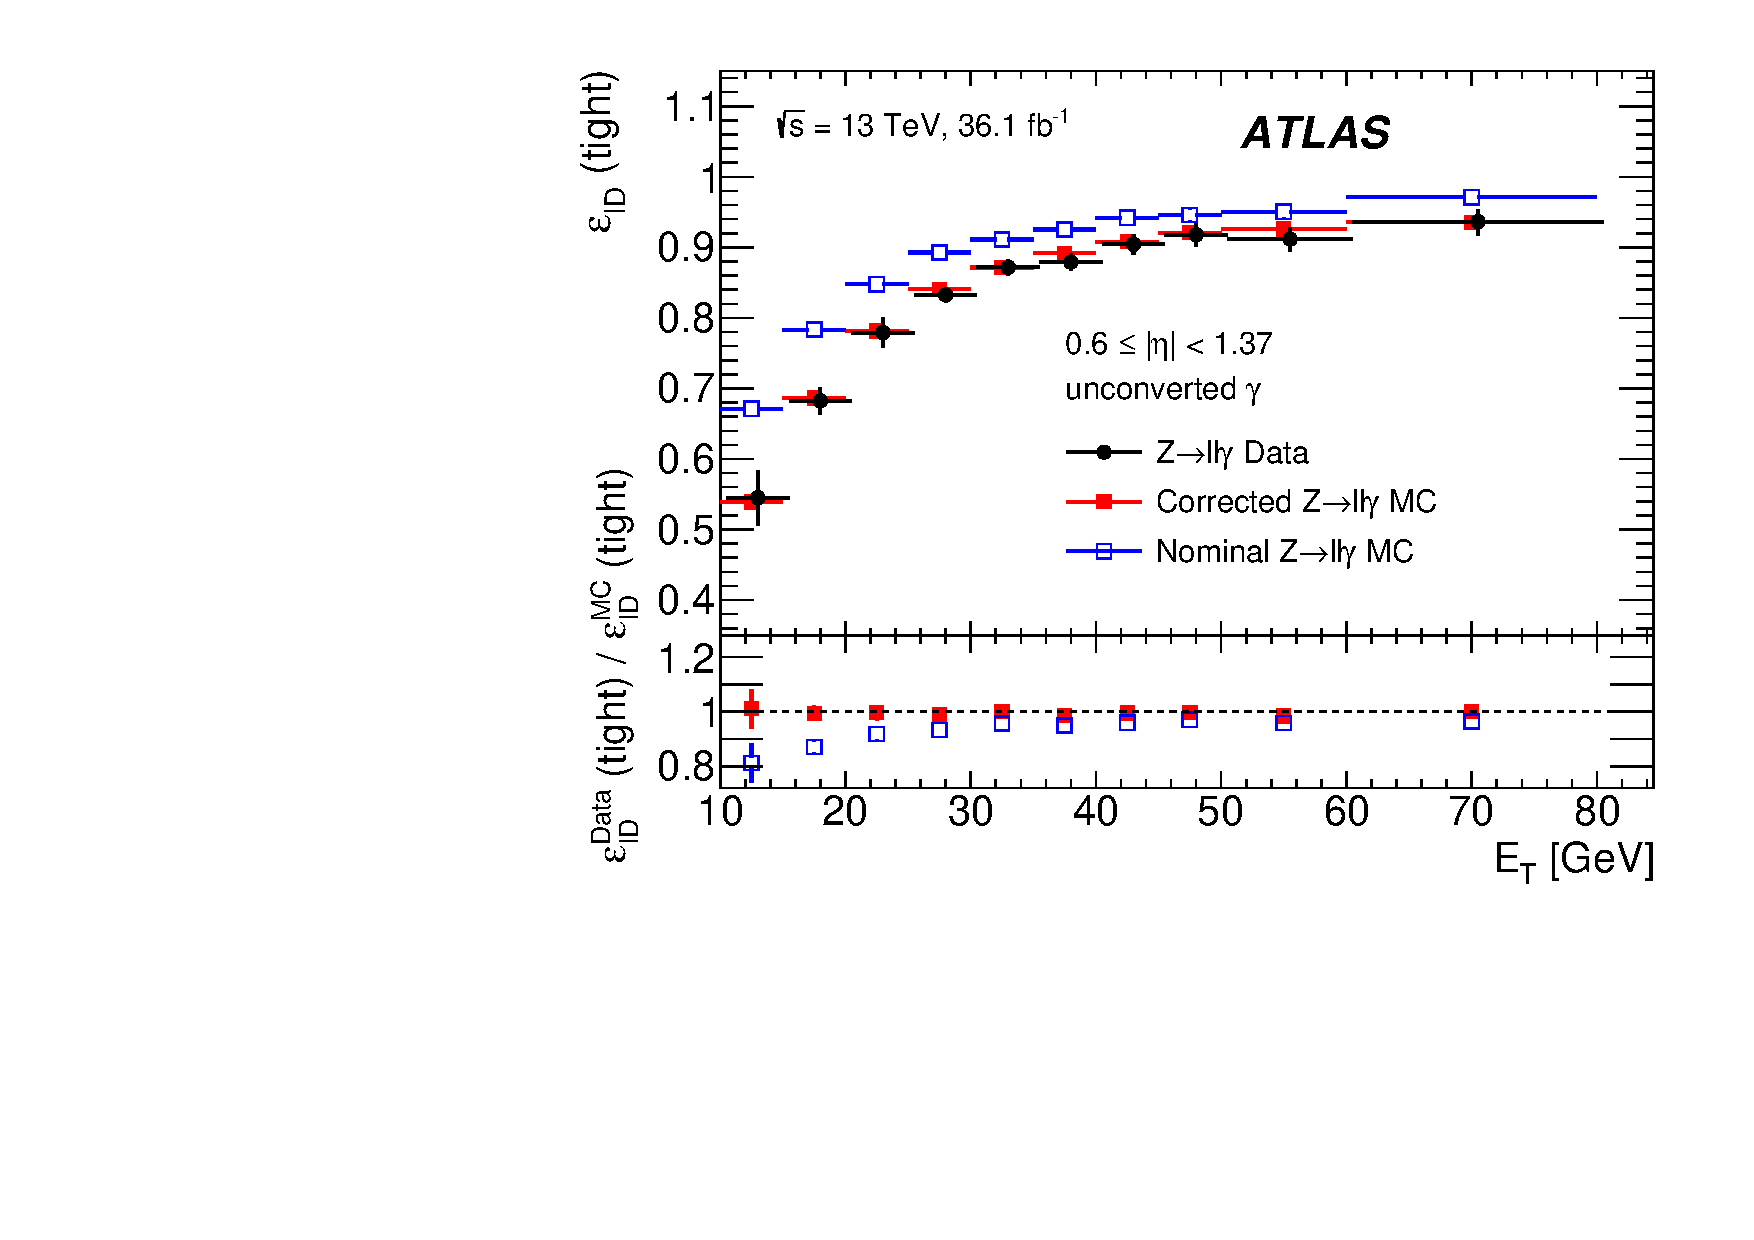
\includegraphics[width=\linewidth]{4_photonid/introduction/efficiencies/pid_rz_efficiency_corrections_comparison}
        \caption{Método \acf{RZ}}
        \label{fig:pid_ss:pid:efficiencies:efficiencies_old:rz}
    \end{subfigure}
    \hfill
    \begin{subfigure}[h]{0.49\linewidth}
        \centering
        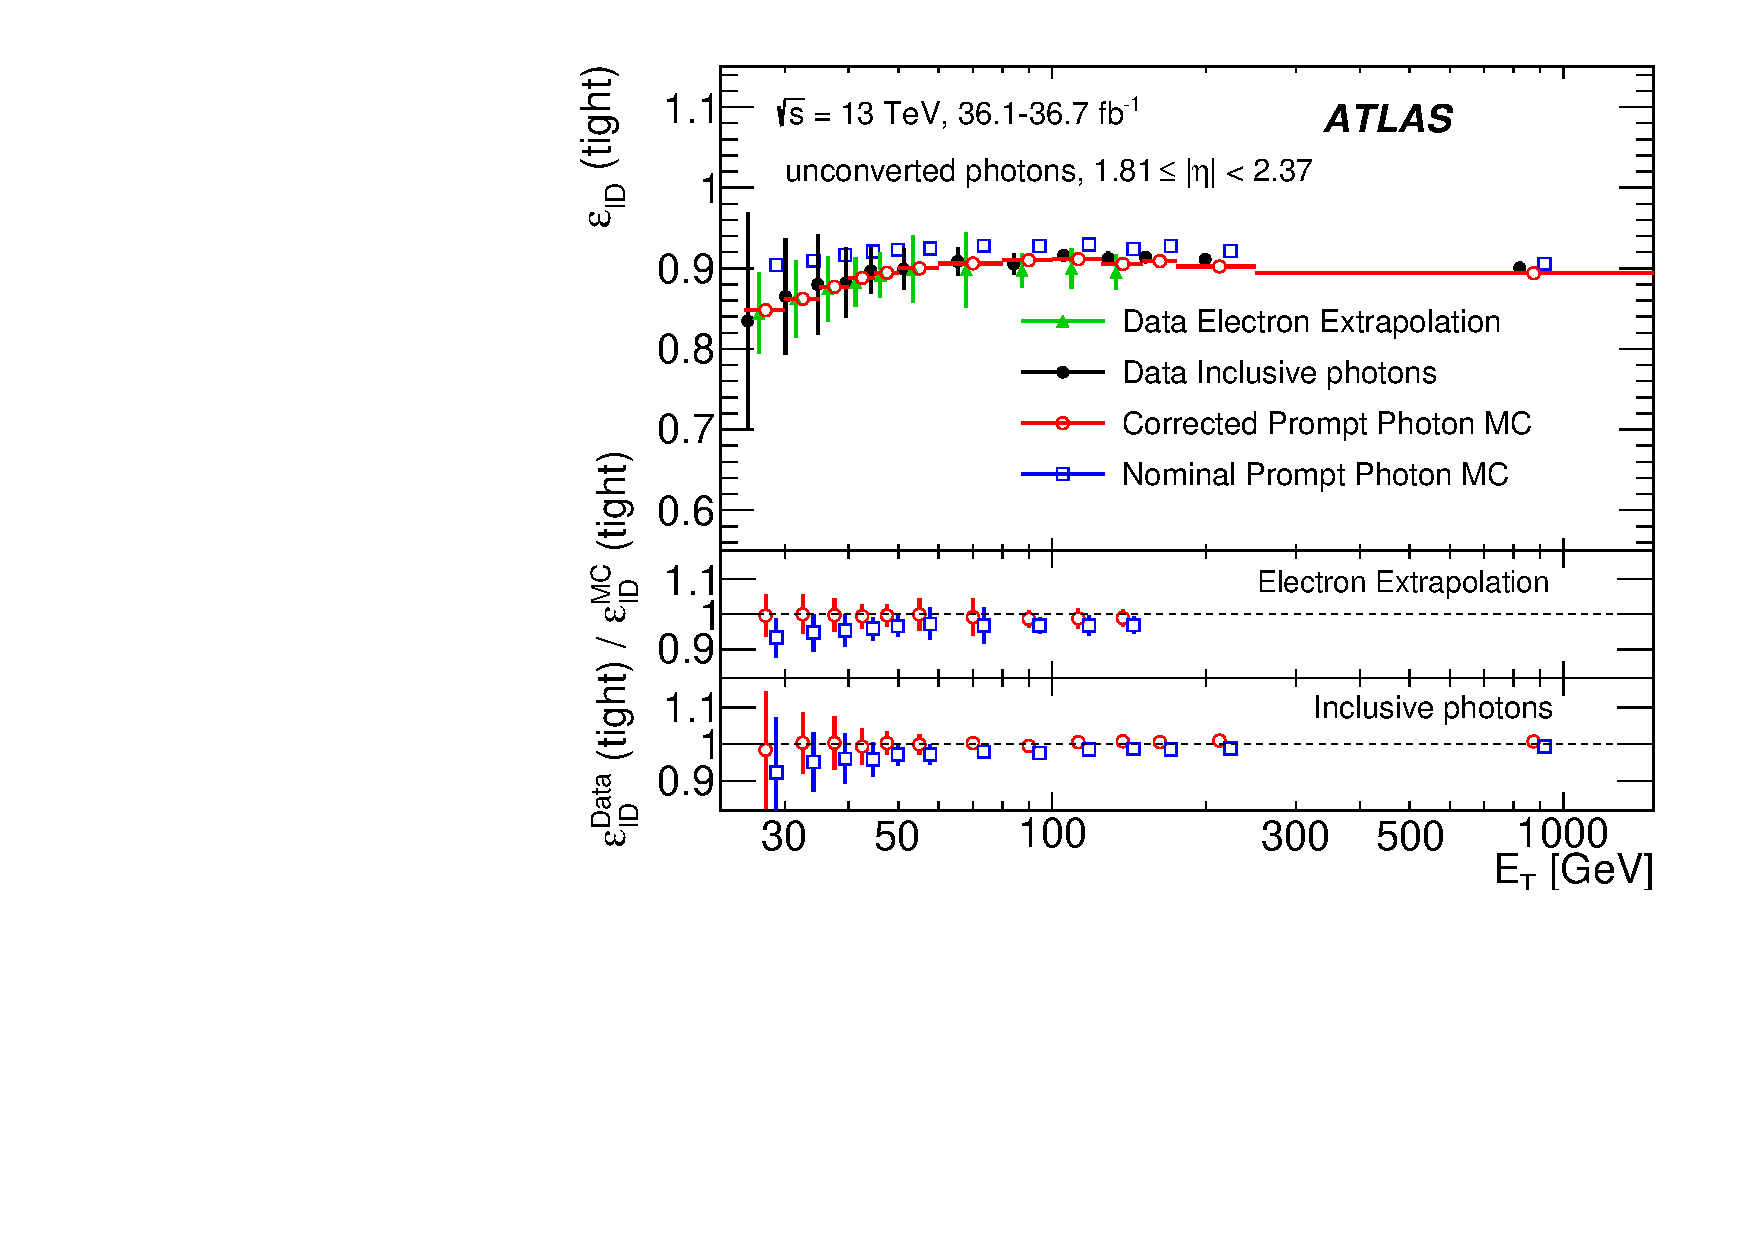
\includegraphics[width=\linewidth]{4_photonid/introduction/efficiencies/pid_ee_sp_efficiency_corrections_comparison}
        \caption{Extrapolación de electrones y Matrix-Method}
        \label{fig:pid_ss:pid:efficiencies:efficiencies_old:ee_sp}
    \end{subfigure}
    \caption{Comparación de las eficiencias calculadas para datos y \ac{MC} utilizando los tres métodos diferentes para su cálculo. En ambas figuras, para cada método, se muestran dos conjuntos diferentes de mediciones \ac{MC}: la nominal y la corregida (discutida en el texto). Los paneles inferiores muestran el cociente entre las eficiencias de los datos y las predicciones \ac{MC} (denominadas \acfp{SF} en el texto). Las figuras fueron tomadas de la \Refn{\cite{ATLAS-EGamma-Performance-2015-2016}}.}
    \label{fig:pid_ss:pid:efficiencies:efficiencies_old}
\end{figure}


En la \Fig{\ref{fig:pid_ss:pid:efficiencies:efficiencies_old:rz}} se muestra un ejemplo de las eficiencias de identificación en función del \pt del fotón utilizando el método \ac{RZ}. Las eficiencias de los datos están representadas por los puntos negros, mientras que el \ac{MC} nominal se muestra con cuadrados azules vacíos. Los cocientes de datos con el \ac{MC} nominal (también denominados \acf{SF}) mostrados en el panel inferior difieren hasta en un 20\% de 1, evidenciando que las eficiencias calculadas con \ac{MC} difiere de las calculadas con los datos. Sin embargo, también se muestra otro conjunto de eficiencias, pertenecientes a simulaciones de \ac{MC} corregidas, mejorando notablemente el acuerdo entre los datos y la simulación, como se ve de los \acp{SF}. La razón por la que se necesitan estas correcciones y cómo se implementaron en \ac{ATLAS} se explica en la siguiente sección (\Sect{\ref{sec:pid_ss:ss_differences}}), y cómo se corrigen en el \Ch{\ref{ch:ss_corrections}}. La \Fig{\ref{fig:pid_ss:pid:efficiencies:efficiencies_old:ee_sp}} muestra las medidas de eficiencia usando los dos métodos restantes (extrapolación de electrones y Matrix Method), donde se obtienen las mismas mejoras en los \acp{SF} cuando se usa la simulación corregida.

Los \acp{SF} se calculan por separado para cada uno de los tres métodos y después se combinan utilizando una media ponderada~\cite{BLUEMethod} en cada \textit{bin} y suponiendo que las incertezas estadísticas y sistemáticas no están correlacionadas entre los métodos. Los resultados actuales de estos \acp{SF}, calculados utilizando el conjunto completo de datos de Run-2, se muestran en la \Fig{\ref{fig:pid_ss:pid:efficiencies:sfs}}. La obtención de los \acp{SF} es de vital importancia ya que luego son factores que se aplican a los eventos de \ac{MC} para ser corregidos y así lograr una comparación justa con los datos recolectados.

\begin{figure}[ht!]
    \centering
    \begin{subfigure}[h]{0.49\linewidth}
        \centering
        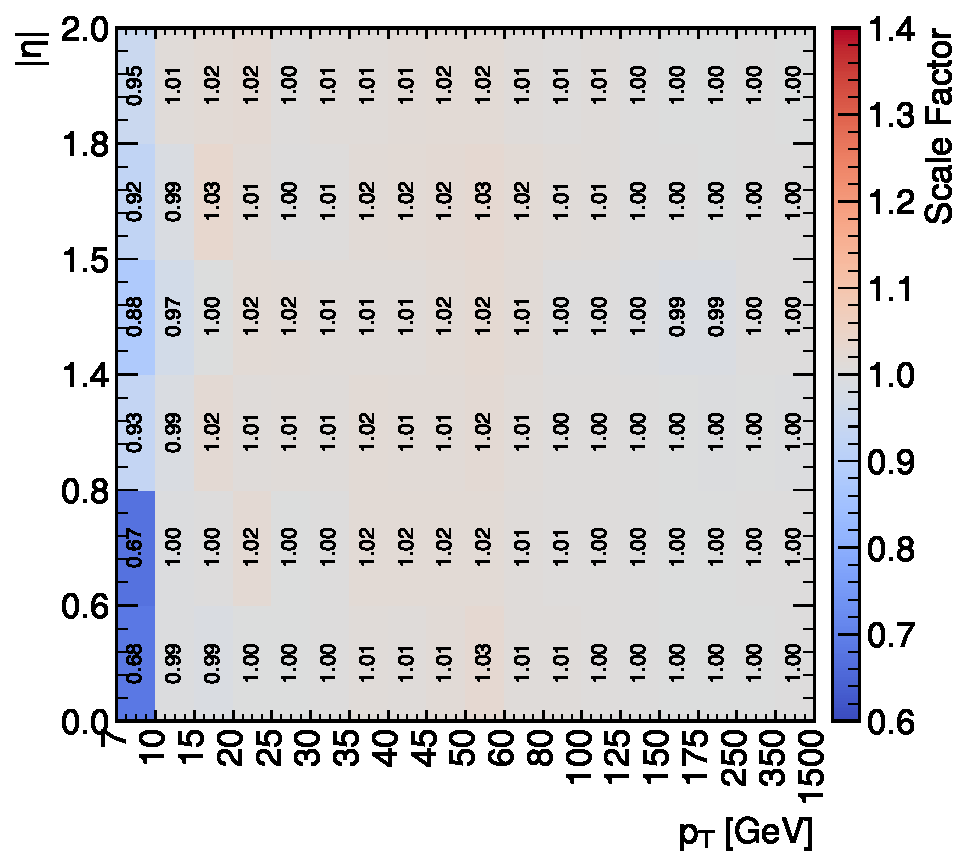
\includegraphics[width=\linewidth]{4_photonid/introduction/efficiencies/sf_pid_c}
        \caption{Fotones convertidos.}
    \end{subfigure}
    \hfill
    \begin{subfigure}[h]{0.49\linewidth}
        \centering
        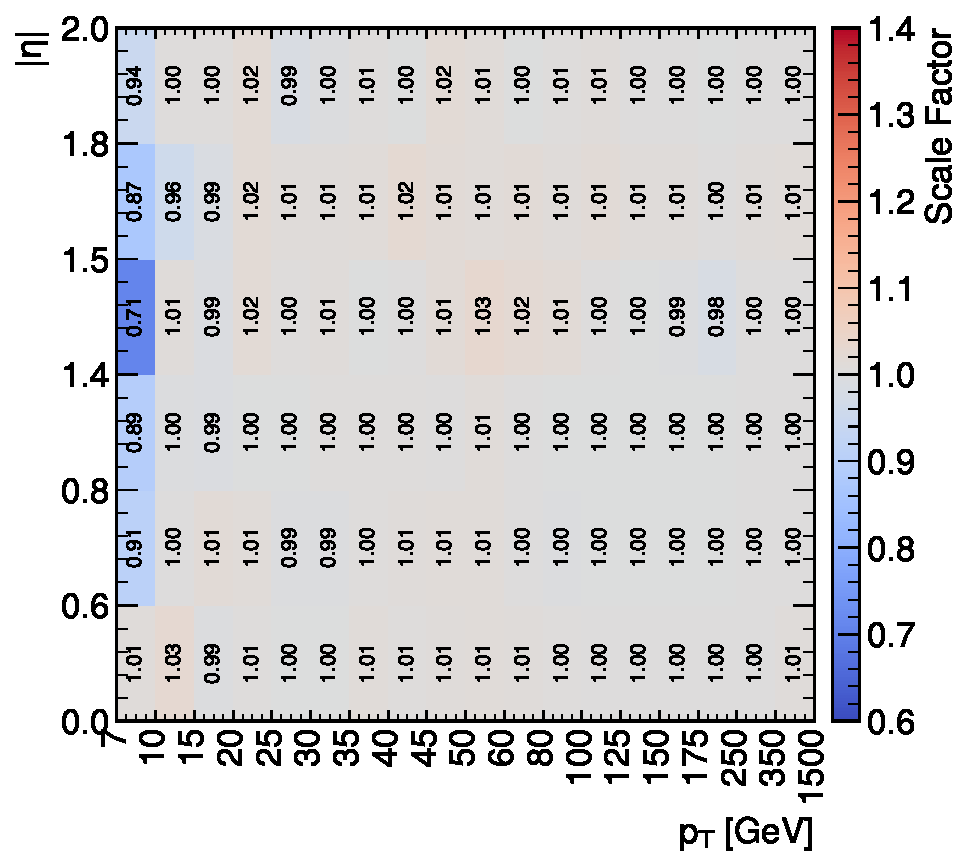
\includegraphics[width=\linewidth]{4_photonid/introduction/efficiencies/sf_pid_unc}
        \caption{Fotones no convertidos.}
    \end{subfigure}
    \caption{\acp{SF} resultantes de la identificación de fotones en los diferentes bines de \pt y \abseta para fotones convertidos (izquierda) and no convertidos (derecha).}
    \label{fig:pid_ss:pid:efficiencies:sfs}
\end{figure}


\section{Las diferencias de las Shower Shapes entre datos y MC}
\label{sec:pid_ss:ss_differences}


Como se ha mostrado anteriormente, la simulación \ac{MC} no describe perfectamente los datos, lo cual puede verse de los valores de los \acp{SF}. En particular, al comparar las distribuciones de las \acp{SS}, se observa que las distribuciones \ac{MC} están desplazadas o incluso la forma difiere, como se muestra en la \Fig{\ref{fig:pid_ss:ss_differences:ss}}, al comparar los datos (puntos negros) con el histograma representado por la línea roja correspondiente al \ac{MC}.

\begin{figure}[ht!]
    \centering
    \begin{subfigure}[h]{0.32\linewidth}
        \centering
        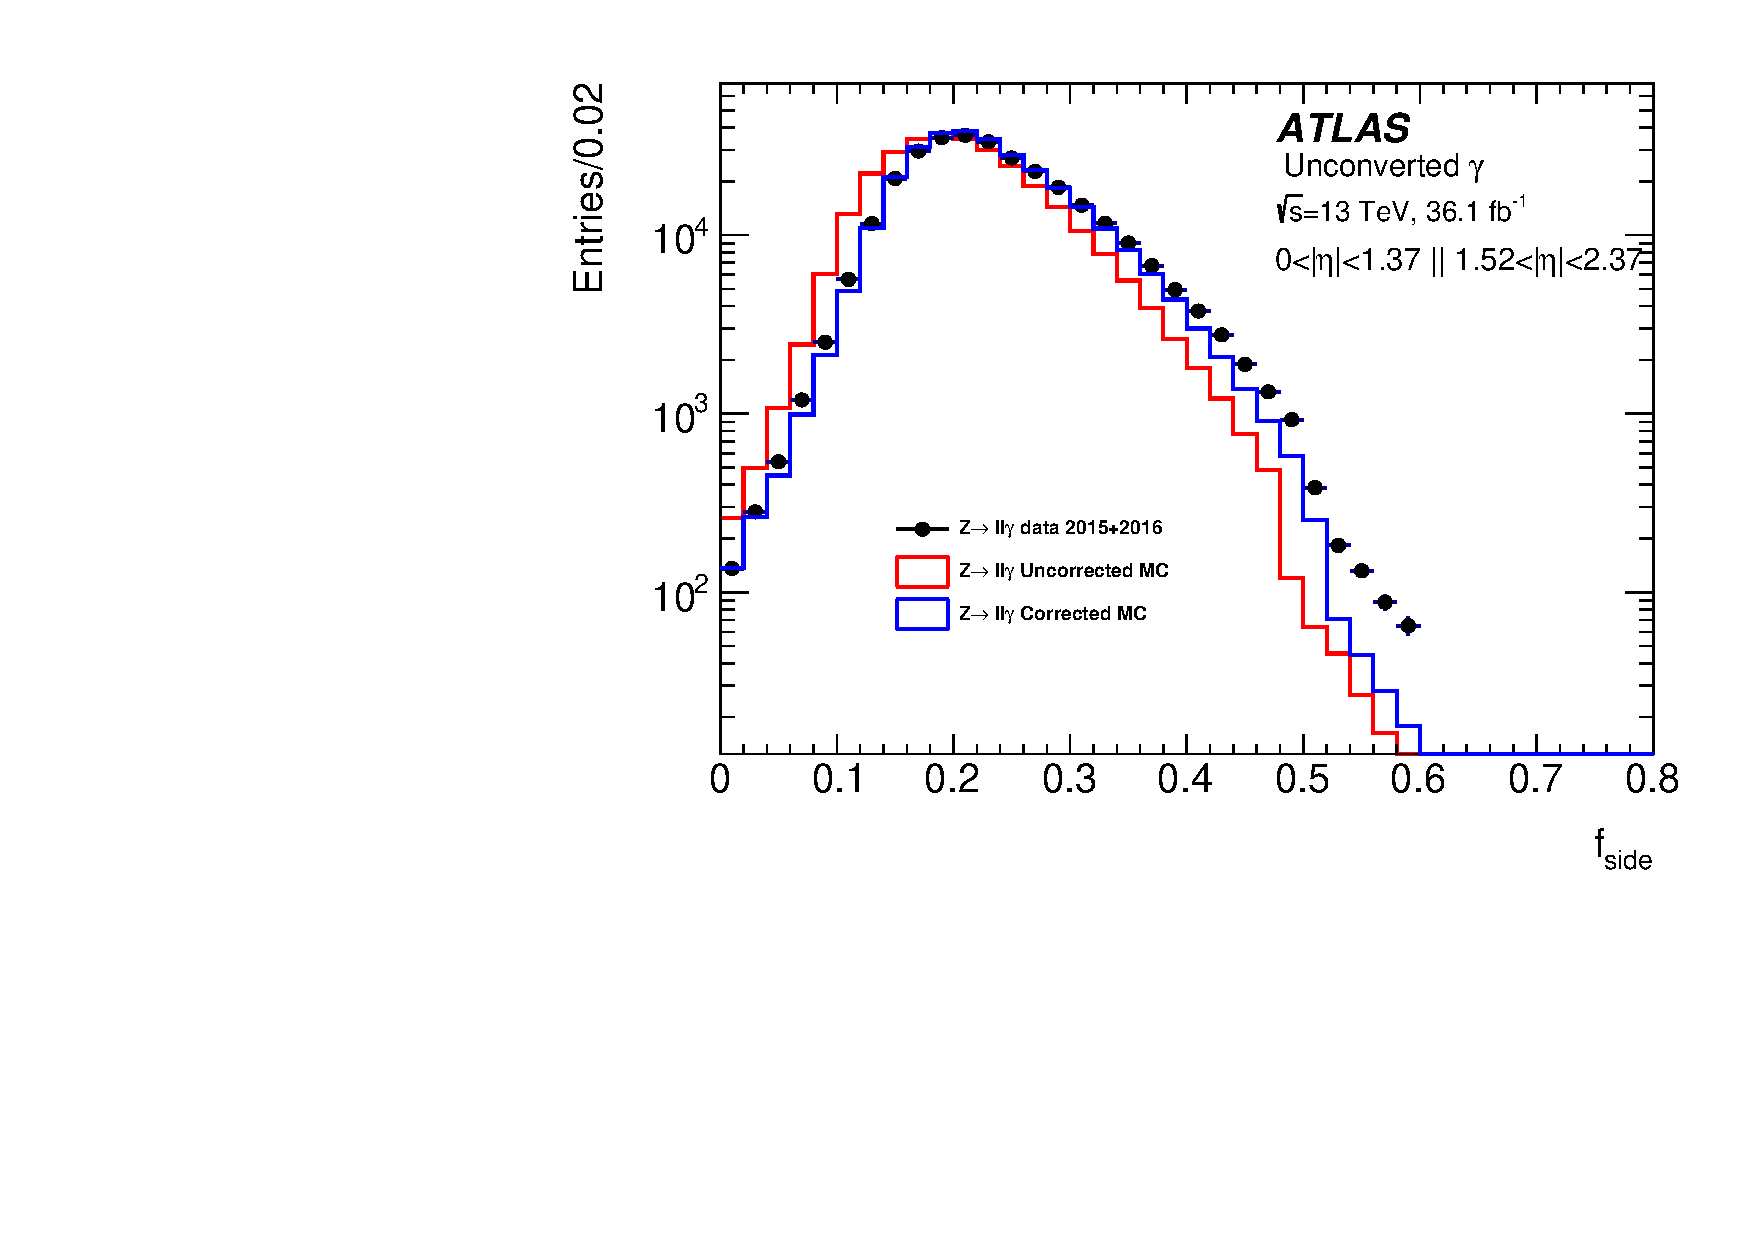
\includegraphics[width=\linewidth]{4_photonid/introduction/shower_shapes/ss_fside_20152016}
        \caption{\fside}
        \label{fig:pid_ss:ss_differences:ss:fside}
    \end{subfigure}
    \hfill
    \begin{subfigure}[h]{0.32\linewidth}
        \centering
        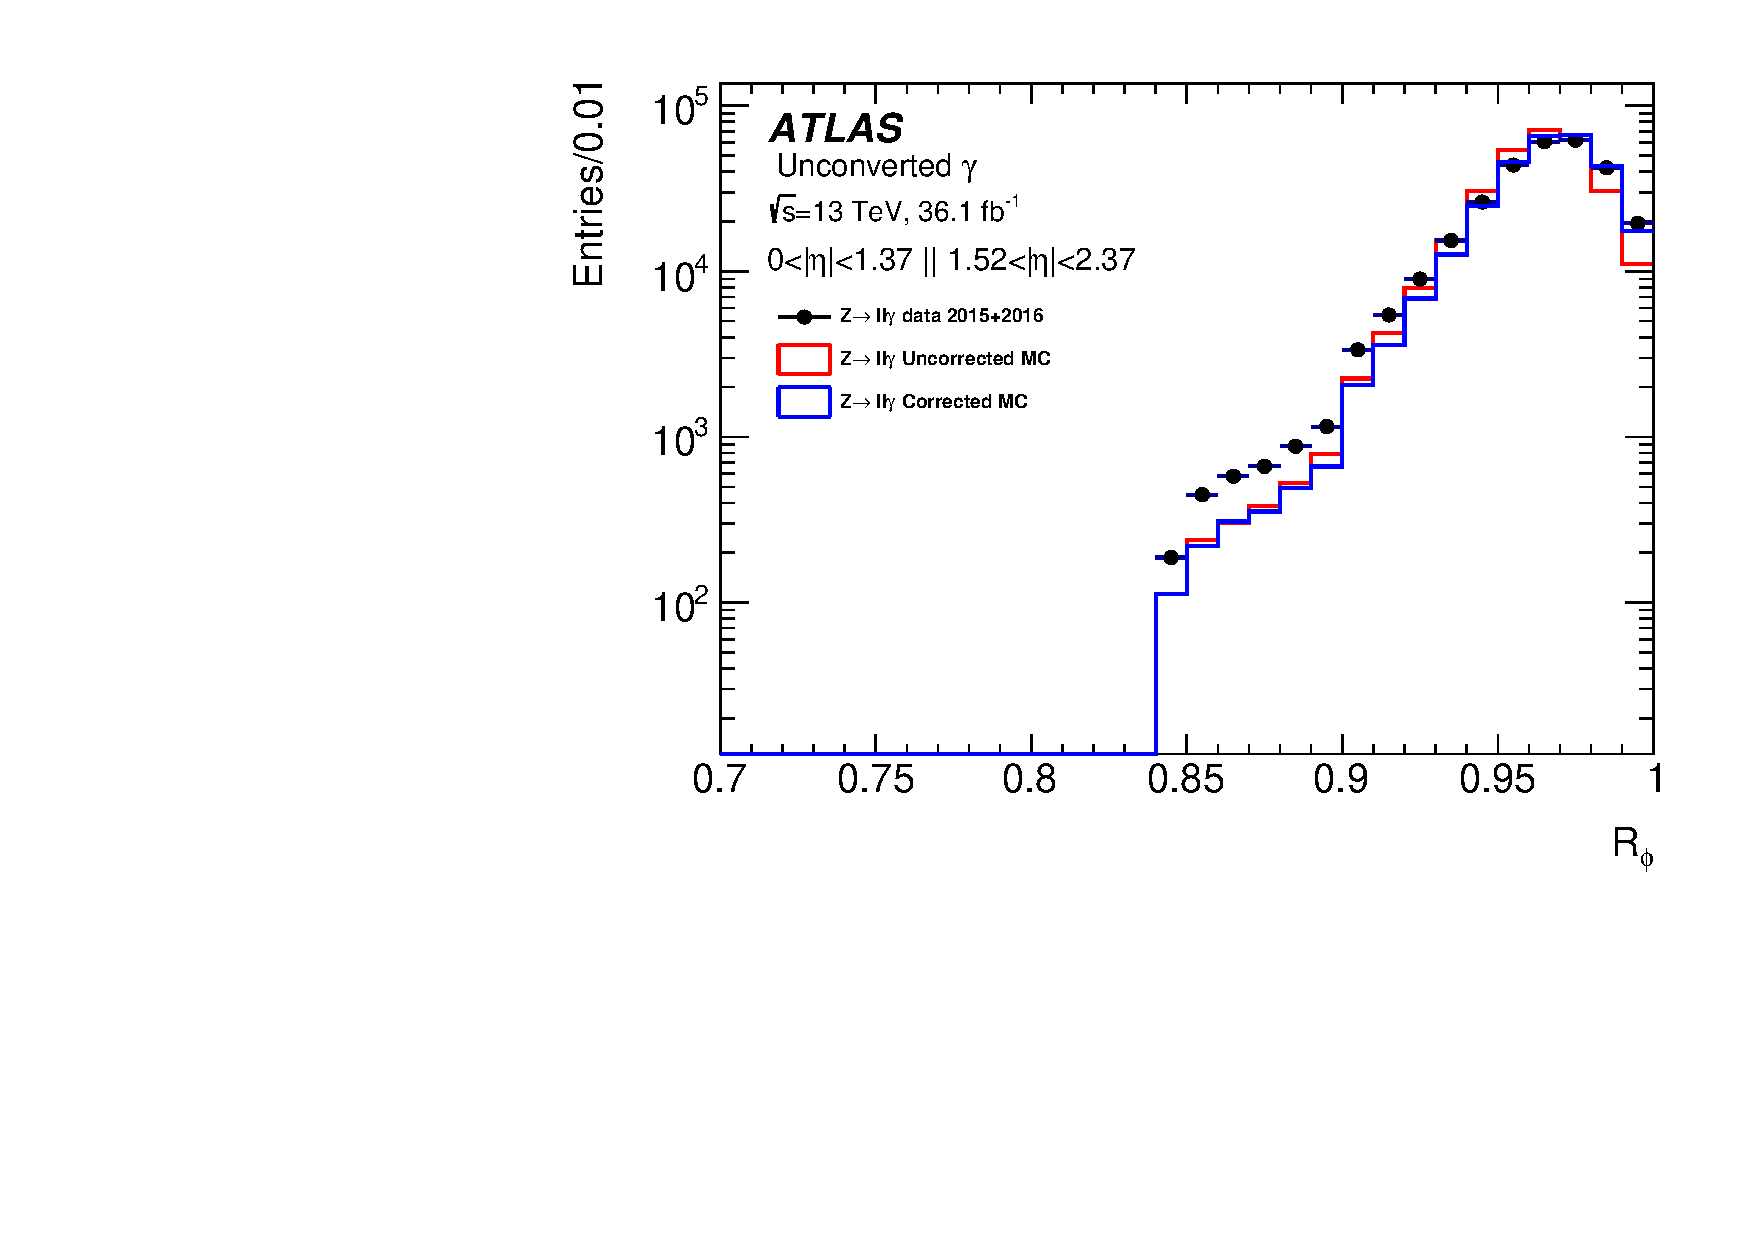
\includegraphics[width=\linewidth]{4_photonid/introduction/shower_shapes/ss_rphi_20152016}
        \caption{\rphi}
        \label{fig:pid_ss:ss_differences:ss:rphi}
    \end{subfigure}
    \hfill
    \begin{subfigure}[h]{0.32\linewidth}
        \centering
        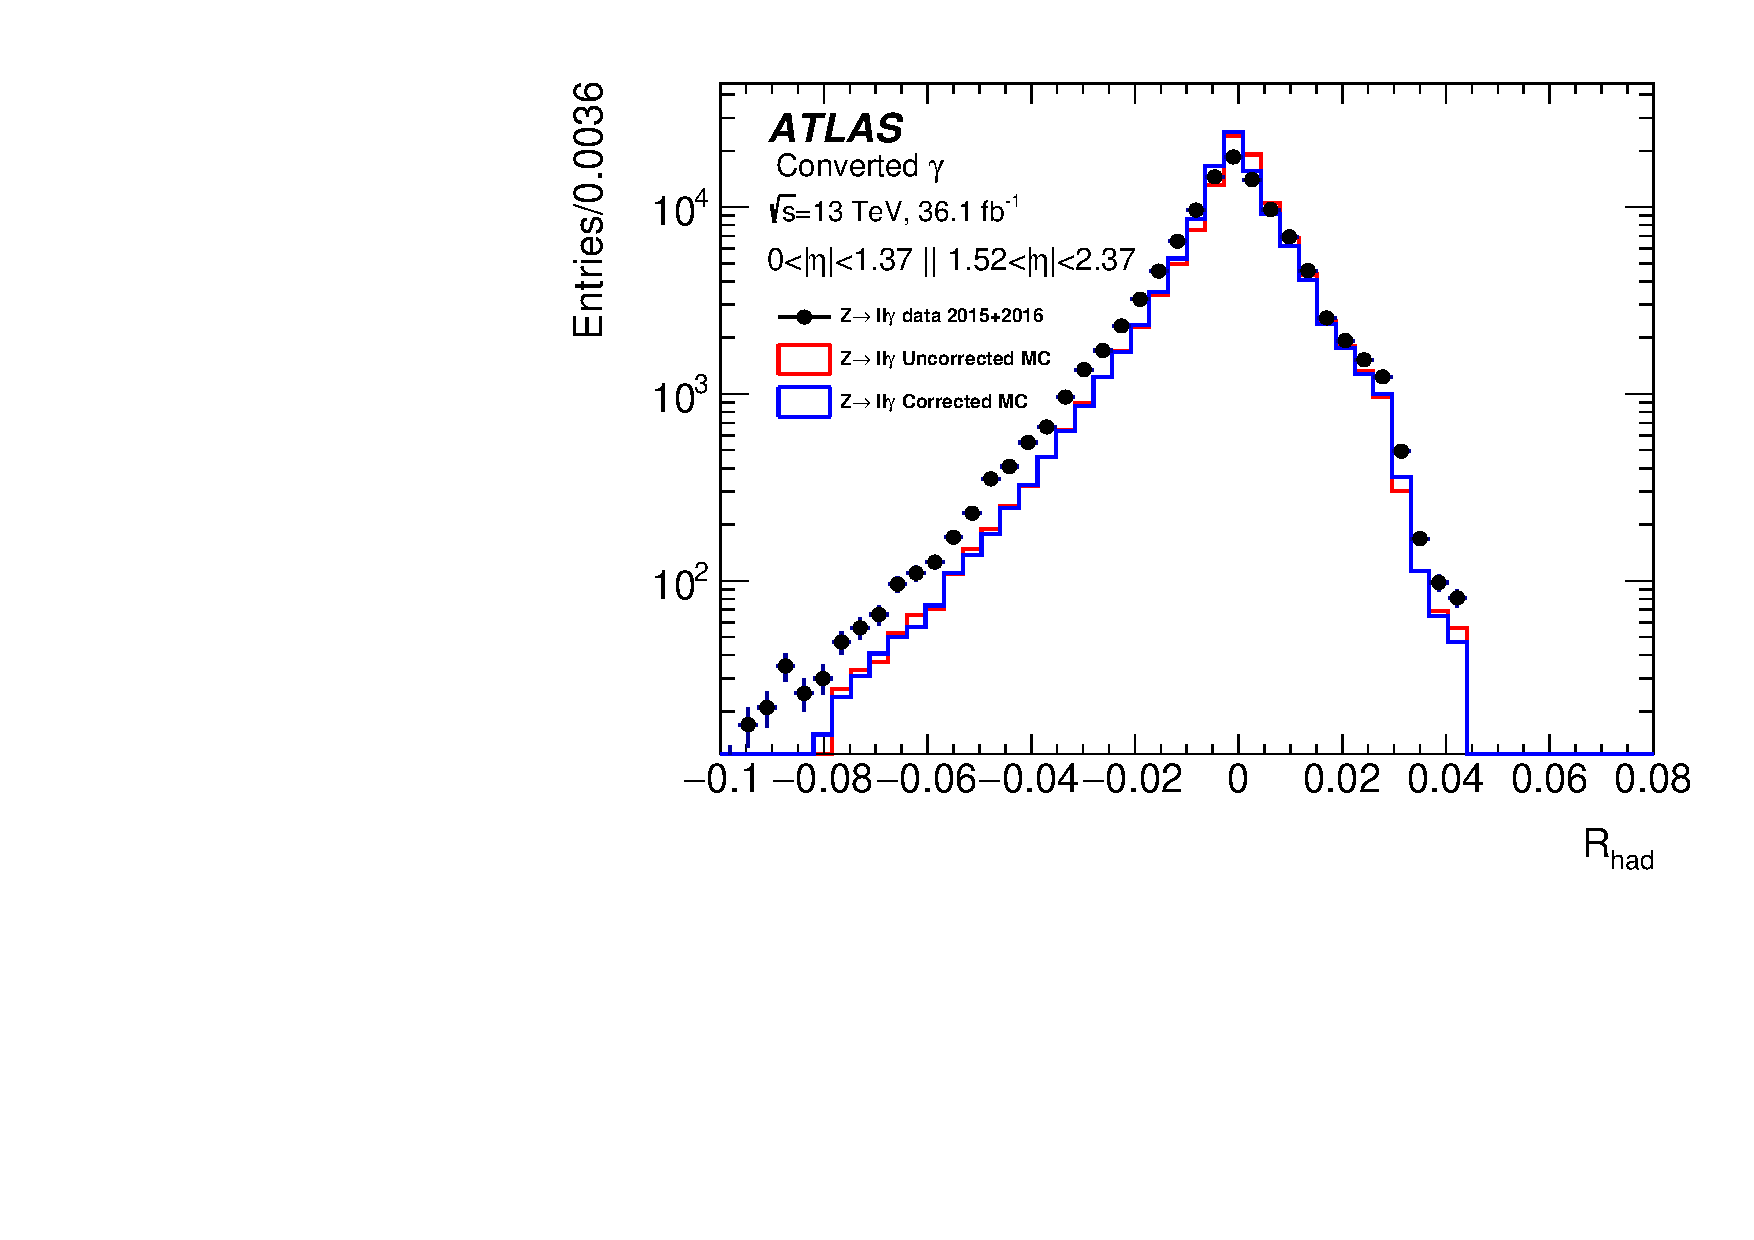
\includegraphics[width=\linewidth]{4_photonid/introduction/shower_shapes/ss_rhad_20152016}
        \caption{\rhad}
        \label{fig:pid_ss:ss_differences:ss:rhad}
    \end{subfigure}
    \caption{Comparación de las \acp{SS} entre los datos (puntos negros) y la simulación \ac{MC} nominal (línea roja) y corregida (línea azul), utilizando la muestra \ac{RZ}~\cite{ATLAS-EGamma-Calibration-2015-2016}.}
    \label{fig:pid_ss:ss_differences:ss}
\end{figure}

Las principales diferencias se observan en los perfiles de la lluvia en la dirección de \(\eta\), donde las distribuciones de datos son más anchas que las de \ac{MC}. Parte del efecto se corrigió en 2010 considerando una descripción detallada de la composición del material absorbente del \ac{ECAL} en \textsc{Geant4}. Sin embargo, algunas discrepancias entre los datos y \ac{MC} aún permanecen y son motivos de estudio para la colaboración. Algunas razones potenciales pueden ser:
\begin{itemize}
    \item Descripción geométrica del grosor del plomo en el \ac{ECAL} (incluyendo posibles variaciones debidas a la gravedad).
    \item Modelado erróneo del campo eléctrico en los huecos de \ac{LAr}.
    \item Modelado erróneo del efecto de \textit{cross-talk} (intercambio de energía entre las celdas del calorímetro debido a la electrónica).
\end{itemize}


Para tener en cuenta estas diferencias en las \acp{SS} de \ac{MC}, históricamente, se realizaban correcciones en forma de desplazamientos de cada una de las distribuciones de \ac{MC}. Estos desplazamientos comprendían los denominados \acfp{FF} y se determinaban utilizando una minimización de \chisq en la comparación de las distribuciones de las \acp{SS} entre datos y \ac{MC}~\cite{ATLAS-EGamma-Performance-2015-2016,ATLAS-EGamma-Performance-2015-2017}.
Aunque las diferencias del valor medio disminuyeron sustancialmente tras estas correcciones, como se observa por ejemplo en el caso de \fside en la \Fig{\ref{fig:pid_ss:ss_differences:ss:fside}}, quedaron diferencias residuales pero aún así notables.
Es evidente que estas diferencias se deben principalmente a la forma de las distribuciones sugiriendo que era necesario realizar una corrección de orden superior.
En el siguiente capítulo se presenta una descripción detallada de las correcciones, realizada como parte de esta tesis.
Además, dado que las \acp{SS} se construyen a partir de depósitos de energía en las celdas del \ac{ECAL}, otra forma posible de mejorar el acuerdo es corregir directamente las energías de las celdas en las simulaciones \ac{MC} y de esta forma todas \acp{SS} se modifican simultáneamente. Este nuevo enfoque se describe también en el siguiente capítulo.